
\section{Empirical Performance Analysis}
\label{interpretability_imli_sec:experiments}
In this section, we empirically evaluate the performance of {\imli}. We first present the experimental setup and the objective of the experiments, followed by experimental results.


\subsection{Experimental Setup}
We implement a prototype of {\imli} in Python to evaluate the performance of the proposed MaxSAT-based formulation for learning classification rules. To implement {\imli}, we deploy a state-of-the-art MaxSAT solver Open-WBO~\cite{martins2014open}, which returns the current best solution upon reaching a timeout. 

We compare {\imli} with state-of-the-art interpretable and non-interpretable classifiers. Among interpretable classifiers, we compare with RIPPER~\cite{cohen1995fast}, BRL~\cite{letham2015interpretable}, CORELS~\cite{angelino2017learning}, and BRS~\cite{wang2017bayesian}. Among non-interpretable classifiers, we compare with Random Forest (RF), Support Vector Machine with linear kernels (SVM), Logistic Regression classifier (LR), and k-Nearest Neighbors classifier (kNN). We deploy the Scikit-learn library in Python for implementing non-interpretable classifiers. 


We experiment with real-world binary classification datasets from  UCI~\cite{Dua:2019}, Open-ML~\cite{OpenML2013}, and Kaggle repository (\url{https://www.kaggle.com/datasets}), as listed in Table~\ref{interpretability_imli_table:interpretable_classifiers}. In these datasets, the number of samples vary from about $ 200 $ to $ 1,000,000 $.  The datasets contain both real-valued and categorical features. We process them to binary features by setting the maximum number of bins as $ 10 $ during discretization. For non-interpretable classifiers such as RF, SVM, LR, and kNN that take real-valued features as inputs, we only convert categorical features to one-hot encoded binary features. 



We perform ten-fold cross-validation on each dataset and evaluate the performance of different classifiers based on the median prediction accuracy on the test data. Additionally, we compare the median size of generated rules among rule-based interpretable classifiers. We consider a comparable combination ($ 100 $) of  hyper-parameters choices for all classifiers, that we fine-tune during cross-validation. For {\imli}, we vary the number of clauses $ k \in \{1, 2, \dots, 5\} $ and the regularization parameter $ \lambda $  in a logarithmic grid by choosing $ 5 $ values between $ 10^{-4} $ and $ 10^1 $. For mini-batch learning in {\imli}, we set the number of samples in each mini-batch, $ n' \in \{50, 100, 200, 400\} $. Thus, we consider $ \lceil n / n' \rceil $ mini-batches, where $ n $ denotes the size of training data. To construct mini-batches from a training dataset, we sequentially split the data into $ \lceil n / n' \rceil $  batches with each batch having $ n' $ samples. Furthermore, to ignore the effect of batch-ordering, we perform mini-batch learning in two rounds such that each batch participates twice in the training.

For BRL algorithm, we vary four hyper-parameters: the maximum cardinality of rules in $ \{2, 3, 4\} $, the minimum support of rules in $ \{0.05, 0.175, 0.3\} $, and the prior on the expected length and width of rules in $ \{2, 4, 6, 8\} $ and $ \{2, 5, 8\} $, respectively. For CORELS algorithm, we vary three hyper-parameters:  the maximum cardinality of rules in $ \{2,, 5\} $, the minimum support of rules in $ \{0.01, 0.17, 0.33, 0.5  \} $, and the regularization parameter in $ \{0.005, 0.01 , 0.015, 0.02 , 0.025, 0.03\}  $. For BRS algorithm, we vary three hyper-parameters: the number of initial rules in $ \{500, 1000, 1500, 2000, 2500, 3000\} $, the maximum length of rules in $ \{1,2,3,4\} $, and the minimum support of rules in $ \{1, 4,7, 10\} $. For RF and RIPPER classifiers, we vary the cut-off on the number of samples in the leaf node using a linear grid between $ 3 $ to $ 500 $ and $ 1 $ to $ 300 $, respectively. For SVM and LR classifiers, we discretize the regularization parameter on a logarithmic grid between  $ 10^{-3} $ and $ 10^3 $. For kNN, we vary the number of neighbors in a linear grid between $ 1 $ and $ 500 $. We conduct each experiment on an Intel Xeon E$ 7-8857 $ v$ 2 $ CPU using a single core with $ 16 $ GB of RAM running on a 64bit Linux distribution based on Debian. For all classifiers, we set the training timeout to $ 1000 $ seconds. 


\paragraph{Objectives of Experiments.} In the following, we present the objectives of our experimental study. 

\begin{enumerate}
	\item How are the accuracy and size of classification rules generated by  {\imli} compared to existing interpretable classifiers?
	\item How is the scalability of {\imli} in solving large-scale classification problems compared to existing interpretable classifiers?
	\item How does {\imli} perform in terms of accuracy and scalability compared to classifiers that are non-interpretable? 
	\item How does the incremental learning in {\imli} perform compared to non-incremental MaxSAT-based learning in terms of accuracy, rule-sparsity, and scalability?
	\item How do different interpretable classification rules learned using {\imli} perform in terms of accuracy and rule-size?
	\item What are the effects of different hyper-parameters in {\imli}?
\end{enumerate} 

\paragraph{Summary of Experimental Results.}
To summarize our experimental results, {\imli} achieves the best balance among prediction accuracy, interpretability, and scalability compared to existing interpretable rule-based classifiers. Particularly, compared to the most accurate classifier RIPPER, {\imli} demonstrates on average $ 1\% $ lower prediction accuracy, wherein the accuracy of {\imli} is higher than BRL, CORELS, and BRS in almost all datasets. In contrast, {\imli} generates significantly smaller rules than RIPPER, specifically in large datasets. Moreover, BRL, CORELS, and BRS report comparatively smaller rule-size than {\imli} on average, but with a significant decrease in accuracy.  In terms of scalability, {\imli} achieves the best performance compared to other interpretable and non-interpretable classifiers by classifying datasets with one million samples. While CORELS also scales to such large datasets,  its accuracy is lower than that of {\imli} by at least $ 2\% $ on average.  Therefore, {\imli} is not only scalable but also accurate in practical classification problems while also being interpretable by design.  We additionally analyze the comparative performance of different formulations presented in this paper, where the  incremental approach empirically proves its efficiency than the na\"ive MaxSAT formulation.  Furthermore, we learn and compare the performance of different interpretable representations: decision lists, decision sets, CNF, and DNF formulas using {\imli} and present the efficacy of {\imli} in learning varied interpretable classifiers. Finally, we study the effect of different hyper-parameters in {\imli}, where each hyper-parameter provides a precise control among training time,  prediction accuracy, and rule-sparsity. In the following, we discuss our experimental results in detail. 




\begin{table*}[!t]
	\centering
	
	\caption[Accuracy and rule-size of interpretable classifiers]{Comparison of accuracy and rule-size among interpretable classifiers. Each cell from the fourth to the eighth column contains test accuracy (top) and rule-size (bottom). `\textemdash' represents a timeout. Numbers in bold represent the best performing results among different classifiers.}
	\label{interpretability_imli_table:interpretable_classifiers} 
	%	\setlength{\tabcolsep}{.2em}
	\small
	\begin{tabular}{lrrrrrrrrrrrr}
		
		
	\toprule
	Dataset & Size & Features & RIPPER & BRL & CORELS & BRS & IMLI \\
	
	\midrule
	\multirow{2}{*}{Parkinsons} & \multirow{2}{*}{ $ 195 $ } & \multirow{2}{*}{ $ 202 $ }  &
	$ 94.44 $  &  $ \mathbf{94.74} $  &  $ 89.74 $  &  $ 84.61 $  &  $ \mathbf{94.74} $  \\
	&&& $ 7.0 $  &  $ 11.5 $  &  $ \mathbf{2.0} $  &  $ 5.0 $  &  $ 7.5 $  \\
	\addlinespace[0.5em]
	
	\multirow{2}{*}{WDBC} & \multirow{2}{*}{ $ 569 $ } & \multirow{2}{*}{ $ 278 $ }  &
	$ \mathbf{98.08} $  &  $ 93.81 $  &  $ 92.04 $  &  $ 92.98 $  &  $ 94.74 $  \\
	&&& $ 13.0 $  &  $ 22.0 $  &  $ \mathbf{2.0} $  &  $ 7.0 $  &  $ 11.5 $  \\
	\addlinespace[0.5em]
	
	\multirow{2}{*}{Pima} & \multirow{2}{*}{ $ 768 $ } & \multirow{2}{*}{ $ 83 $ }  &
	$ 77.14 $  &  $ 68.18 $  &  $ 75.32 $  &  $ 75.32 $  &  $ \mathbf{78.43} $  \\
	&&& $ 6.0 $  &  $ 13.5 $  &  $ \mathbf{2.0} $  &  $ 3.0 $  &  $ 23.0 $  \\
	\addlinespace[0.5em]
	
	\multirow{2}{*}{Titanic} & \multirow{2}{*}{ $ 1,043 $ } & \multirow{2}{*}{ $ 38 $ }  &
	$ 78.72 $  &  $ 62.98 $  &  $ \mathbf{81.9} $  &  $ 80.86 $  &  $ 81.82 $  \\
	&&& $ 6.0 $  &  $ 15.0 $  &  $ \mathbf{4.0} $  &  $ \mathbf{4.0} $  &  $ 5.5 $  \\
	\addlinespace[0.5em]
	
	\multirow{2}{*}{MAGIC} & \multirow{2}{*}{ $ 19,020 $ } & \multirow{2}{*}{ $ 100 $ }  &
	$ \mathbf{82.68} $  &  $ 76.95 $  &  $ 78.05 $  &  $ 77.5 $  &  $ 78.26 $  \\
	&&& $ 102.0 $  &  $ 81.0 $  &  $ 4.0 $  &  $ \mathbf{3.0} $  &  $ 8.5 $  \\
	\addlinespace[0.5em]
	
	\multirow{2}{*}{Tom's HW} & \multirow{2}{*}{ $ 28,179 $ } & \multirow{2}{*}{ $ 946 $ }  &
	$ \mathbf{85.91} $  & \textemdash &  $ 83.27 $  &  $ 83.13 $  &  $ 85.24 $  \\
	&&& $ 30.0 $  & \textemdash &  $ \mathbf{4.0} $  &  $ 18.5 $  &  $ 44.5 $  \\
	\addlinespace[0.5em]
	
	\multirow{2}{*}{Credit} & \multirow{2}{*}{ $ 30,000 $ } & \multirow{2}{*}{ $ 199 $ }  &
	$ \mathbf{82.39} $  &  $ 46.12 $  &  $ 81.18 $  &  $ 80.45 $  &  $ 82.12 $  \\
	&&& $ 32.5 $  &  $ 26.5 $  &  $ \mathbf{2.0} $  &  $ 7.0 $  &  $ 17.5 $  \\
	\addlinespace[0.5em]
	
	\multirow{2}{*}{Adult} & \multirow{2}{*}{ $ 32,561 $ } & \multirow{2}{*}{ $ 94 $ }  &
	$ \mathbf{84.37} $  &  $ 72.08 $  &  $ 79.78 $  &  $ 70.75 $  &  $ 81.2 $  \\
	&&& $ 115.5 $  &  $ 46.5 $  &  $ \mathbf{4.0} $  &  $ \mathbf{4.0} $  &  $ 30.0 $  \\
	\addlinespace[0.5em]
	
	\multirow{2}{*}{Bank Marketing} & \multirow{2}{*}{ $ 45,211 $ } & \multirow{2}{*}{ $ 82 $ }  &
	$ \mathbf{90.01} $  &  $ 84.66 $  &  $ 89.62 $  &  $ 86.75 $  &  $ 89.84 $  \\
	&&& $ 36.5 $  &  $ 13.0 $  &  $ \mathbf{2.0} $  &  $ \mathbf{2.0} $  &  $ 24.5 $  \\
	\addlinespace[0.5em]
	
	\multirow{2}{*}{Connect-4} & \multirow{2}{*}{ $ 67,557 $ } & \multirow{2}{*}{ $ 126 $ }  &
	$ \mathbf{76.72} $  &  $ 65.83 $  &  $ 68.68 $  &  $ 70.49 $  &  $ 75.36 $  \\
	&&& $ 118.0 $  &  $ 18.5 $  &  $ \mathbf{4.0} $  &  $ 11.0 $  &  $ 50.5 $  \\
	\addlinespace[0.5em]
	
	\multirow{2}{*}{Weather AUS} & \multirow{2}{*}{ $ 107,696 $ } & \multirow{2}{*}{ $ 169 $ }  &
	$ \mathbf{84.22} $  &  $ 43.26 $  &  $ 83.67 $  & \textemdash &  $ 83.78 $  \\
	&&& $ 26.0 $  &  $ 22.0 $  &  $ \mathbf{2.0} $  & \textemdash &  $ 22.0 $  \\
	\addlinespace[0.5em]
	
	\multirow{2}{*}{Vote} & \multirow{2}{*}{ $ 131,072 $ } & \multirow{2}{*}{ $ 16 $ }  &
	$ \mathbf{97.12} $  &  $ 94.78 $  &  $ 95.86 $  &  $ 95.14 $  &  $ 96.69 $  \\
	&&& $ 132.0 $  &  $ 41.5 $  &  $ 3.5 $  &  $ \mathbf{1.0} $  &  $ 15.0 $  \\
	\addlinespace[0.5em]
	
	\multirow{2}{*}{Skin Seg} & \multirow{2}{*}{ $ 245,057 $ } & \multirow{2}{*}{ $ 30 $ }  &
	\textemdash &  $ 79.25 $  &  $ 91.62 $  &  $ 68.48 $  &  $ \mathbf{94.71} $  \\
	&&&\textemdash &  $ 6.0 $  &  $ 9.0 $  &  $ \mathbf{5.0} $  &  $ 30.0 $  \\
	\addlinespace[0.5em]
	
	\multirow{2}{*}{BNG(labor)} & \multirow{2}{*}{ $ 1,000,000 $ } & \multirow{2}{*}{ $ 89 $ }  &
	\textemdash & \textemdash &  $ 88.56 $  & \textemdash &  $ \mathbf{90.91} $  \\
	&&&\textemdash & \textemdash &  $ \mathbf{2.0} $  & \textemdash &  $ 24.0 $  \\
	\addlinespace[0.5em]
	
	\multirow{2}{*}{BNG(credit-g)} & \multirow{2}{*}{ $ 1,000,000 $ } & \multirow{2}{*}{ $ 97 $ }  &
	\textemdash & \textemdash &  $ 72.08 $  & \textemdash &  $ \mathbf{75.48} $  \\
	&&&\textemdash & \textemdash &  $ \mathbf{2.0} $  & \textemdash &  $ 27.5 $  \\
	\bottomrule
	
		
	\end{tabular}

\end{table*}





\subsection{Experimental Results}

\paragraph{Comparing {\imli} with interpretable classifiers.} We compare {\imli} with existing interpretable classifiers in three aspects: test accuracy, rule-size, and scalability.

\textit{Test accuracy and rule-size.}  We present the experimental  results of test accuracy and rule-size among interpretable classifiers in Table~\ref{interpretability_imli_table:interpretable_classifiers}, where the first, second, and third columns represent  the name of the dataset, the number of samples, and the number of features in the dataset, respectively. In each cell from the fourth to the eighth column in the table, the top value represents the median test accuracy and the bottom value represents the median size of rules measured through ten-fold cross-validation. 



In Table~\ref{interpretability_imli_table:interpretable_classifiers}, {\imli} and CORELS generate interpretable classification rules in all $ 15 $ datasets in our experiments. In contrast, within a timeout of $ 1000 $ seconds, RIPPER, BRL, and BRS fail to generate any classification rule in three datasets,  specifically in large datasets ($ \ge 200,000 $ samples). 



We now compare {\imli} with each interpretable classifier in detail. Compared to RIPPER, {\imli} has lower accuracy in $ 9 $ out  of $ 12 $ datasets. More specifically, the accuracy of {\imli} is $ 1\% $ lower on average than RIPPER. The improved accuracy of RIPPER, however, results in the generation of higher size classification rules than {\imli} in most datasets. In particular, {\imli} generates sparser rules than RIPPER in $ 9 $ out of $ 12 $ datasets, wherein RIPPER times out in $ 3 $ datasets. Interestingly, the difference in rule-size is more significant in larger datasets, such as in `Vote' dataset, where RIPPER learns a classifier with $ 132 $ Boolean predicates compared to $ 15 $ Boolean predicates by {\imli}.  Therefore, {\imli} is better than RIPPER in terms of rule-sparsity, but lags slightly in accuracy.


{\imli} performs better than BRL both in terms of accuracy and rule-sparsity. In particular, {\imli} has  higher accuracy and lower rule-size than BRL in $ 12 $ and $ 8 $ datasets, respectively, in a total of $ 12 $ datasets, wherein BRL times out in $ 3 $ datasets.  While comparing with CORELS, {\imli} achieves higher accuracy in almost all datasets ($ 14 $ out of $ 15 $ datasets). A similar trend is observed in comparison with BRS, where {\imli} achieves higher accuracy in all of $ 12 $ datasets and BRS times out in $ 3 $ datasets. CORELS and BRS, however, generates sparser rules than {\imli} in most datasets, but by costing a significant decrease in accuracy.  For example, in the largest dataset `BNG(credit-g)' with $ 1 $ Million samples, BRS times out and CORELS generates a classifier with  $ 72.08\% $ accuracy with rule-size $ 2 $. {\imli}, in contrast, learns a classifier with $ 27.5 $ Boolean predicates achieving $ 75.48\% $ accuracy, which is $ 3\% $ higher than CORELS. Therefore, {\imli}  makes a good balance between accuracy and rule-size compared to existing interpretable classifiers while also being highly scalable. In the following, we discuss the results on the scalability of all interpretable classifiers in detail. 



\textit{Scalability.} We analyze the scalability among interpretable classifiers by comparing their training time. In Figure~\ref{interpretability_imli_fig:interpretable_classifiers}, we use cactus plots\footnote{Cactus plots are often used in (Max)SAT community to present the scalability of different solvers/methods~\cite{argelich2008first,balyo2017sat}.} to represent the training time (in seconds) of all classifiers in $ 1000 $ instances ($ 10 $ folds $ \times  $ $ 100 $ choices of hyper-parameters) derived for each dataset. In the cactus plot, the number of solved instances (within $ 1000 $ seconds) is on the $ X $-axis, whereas the training time is  on the $ Y $-axis. A point $ (x,y) $ on the plot implies that a classifier yields lower than or equal to $ y $ seconds of training in $ x $ many instances. 


In Figure~\ref{interpretability_imli_fig:interpretable_classifiers}, we present results in an increasing number of samples in a dataset (from left to right).
In WDBC and Adult datasets presented on the first two plots in Figure~\ref{interpretability_imli_fig:interpretable_classifiers}, CORELS solves lower than $  600 $ instances within a timeout of $ 1000 $ seconds. The scalability performance of BRS is even worse, where it solves around $ 700 $ and $ 200 $ instances in WDBC and Adult datasets, respectively. The other three classifiers: {\imli}, BRL, and RIPPER  solve all $ 1000 $ instances, where BRL takes comparatively higher training time than the other two. The performance of {\imli} and RIPPER is similar, with RIPPER being comparatively better in the two datasets. However, the efficiency of {\imli} compared to other classifiers becomes significant as the number of samples in a dataset increases. In particular, in `Weather AUS' dataset, BRS cannot solve a single instance, BRL and CORELS solves $ ~400 $ instances, and RIPPER solves around $ 600 $ instances. {\imli}, however, solves all $ 1000 $ instances in this dataset. Similarly, in `BNG(labor)' dataset, all other classifiers except {\imli} and CORELS cannot solve any instance. While {\imli} mostly takes the maximum allowable time ($ 1000 $ seconds) in solving all instances in this dataset, CORELS can solve lower than $ 400 $ instances. 
Thus, {\imli} establishes itself as the most scalable classifier compared to other state-of-the-art interpretable classifiers.


\begin{figure}[!t]
	
	\centering
	
	\subfloat{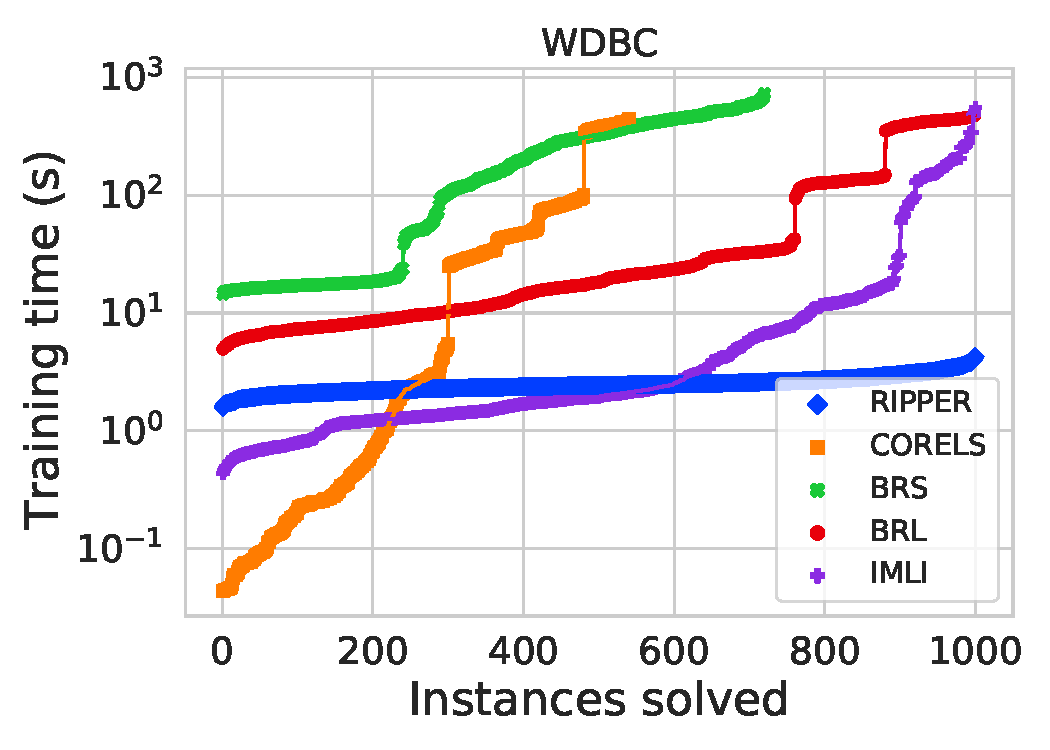
\includegraphics[scale=0.35]{figures/interpretability/imli/dataset_wdbc_cactus_train_val_fit_time}}
	\subfloat{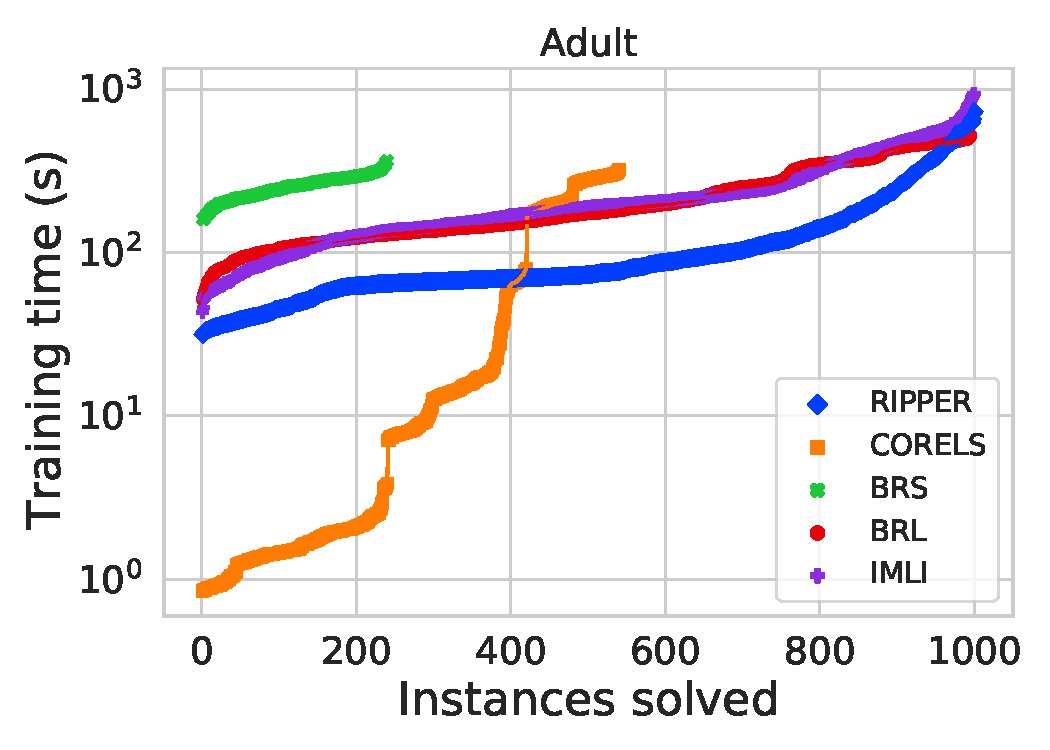
\includegraphics[scale=0.35]{figures/interpretability/imli/dataset_adult_cactus_train_val_fit_time}}\\
	\subfloat{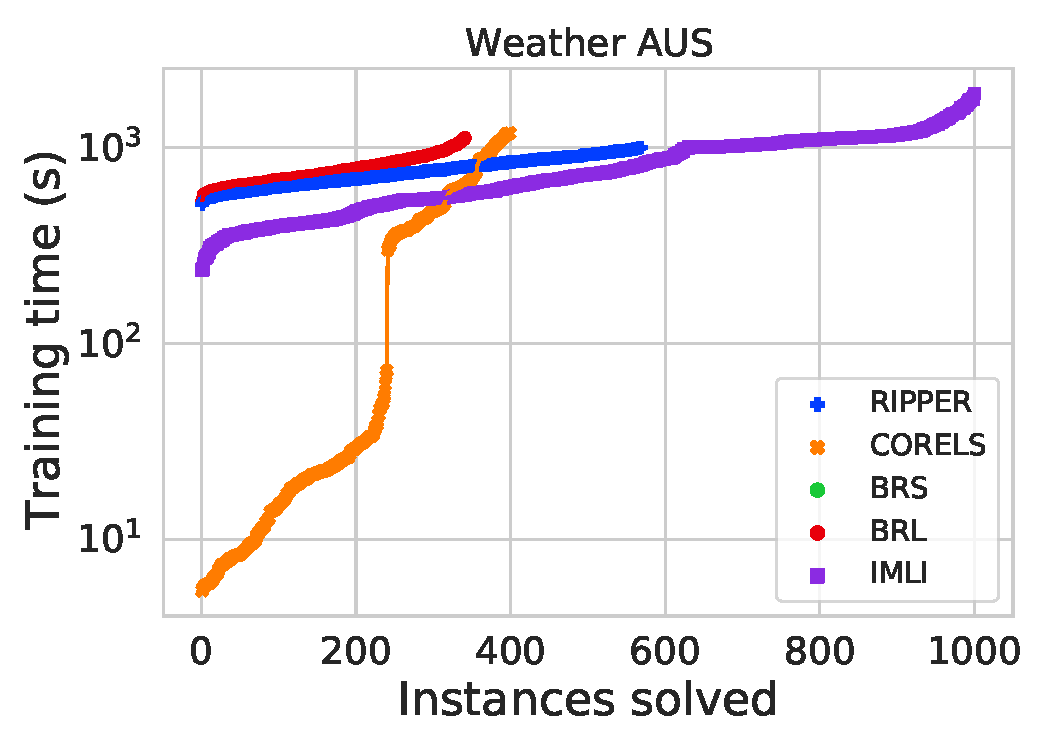
\includegraphics[scale=0.35]{figures/interpretability/imli/dataset_weatherAUS_cactus_train_val_fit_time}}
	\subfloat{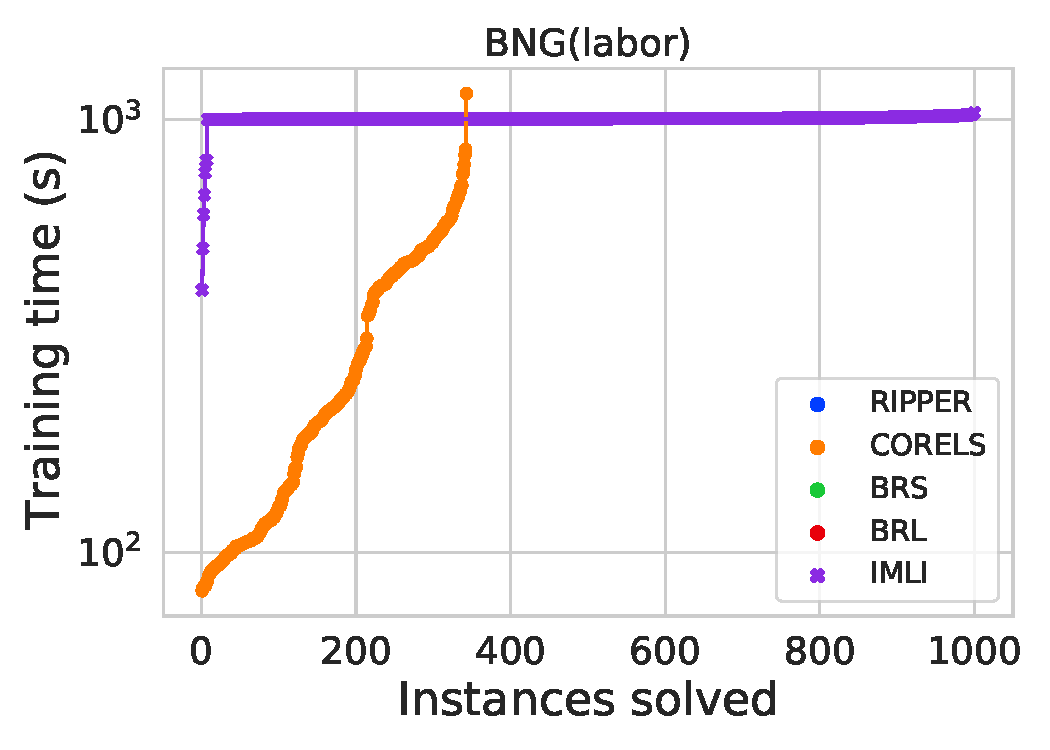
\includegraphics[scale=0.35]{figures/interpretability/imli/dataset_labor_cactus_train_val_fit_time}}
	
	\caption[Scalability of Interpretable Classifiers]{Comparison of scalability among interpretable classifiers. The plots are arranged in increasing sizes of datasets (from left to right). In each cactus plot, {\imli} solves all $ 1000 $ instances for each dataset, while competitive classifiers often fail to scale, specially in larger datasets.}
	\label{interpretability_imli_fig:interpretable_classifiers}
\end{figure}






\paragraph{Comparison with non-interpretable classifiers.} We compare {\imli} with state-of-the-art non-interpretable classifiers such as LR, SVM, kNN, and RF in terms of their median test accuracy in Table~\ref{interpretability_imli_table:non_interpretable_classifiers}. In the majority of the datasets, {\imli} achieves comparatively lower test accuracy than the best performing non-interpretable classifier. The decrease in the test accuracy of {\imli} is attributed to two factors. Firstly, while we train {\imli} on discretized data, non-interpretable classifiers are trained on non-discretized data and thus {\imli} incurs additional classification errors due to discretization. Secondly, {\imli} learns a rule-based classifier, whereas non-interpretable classifiers can learn more flexible decision boundaries and thus fit data well. In Table~\ref{interpretability_imli_table:non_interpretable_classifiers}, we also observe that {\imli} achieves impressive scalability than competing classifiers by solving datasets with $ 1, 000,000 $  samples where most of the non-interpretable classifiers fail to learn any decision boundary on such large datasets. Thus, {\imli}, being an interpretable classifier, demonstrates lower accuracy than competing non-interpretable classifiers, but higher scalability in practice. 


\begin{table*}[!t]        
	\centering
	\caption[Accuracy of {\imli} and non-interpretable classifiers]{Comparison of {\imli} with non-interpretable classifiers in terms of test accuracy. In the table, `\textemdash' represents a timeout. Numbers in bold represent the best performing results among different classifiers.}
	\label{interpretability_imli_table:non_interpretable_classifiers}
	%	\setlength{\tabcolsep}{.2em}
	\small
	\begin{tabular}{lrrrrrrrrrrrrrrr}
		
		
		
		
		\toprule
		Dataset & Size & LR & SVM & kNN & RF & IMLI \\
		
		\midrule
		\multirow{1}{*}{Parkinsons} & \multirow{1}{*}{ $ 195 $ }  &
		$ 89.74 $  &  $ 89.74 $  &  $ \mathbf{97.5} $  &  $ 90.0 $  &  $ 94.74 $  \\
		\multirow{1}{*}{WDBC} & \multirow{1}{*}{ $ 569 $ }  &
		$ \mathbf{98.25} $  &  $ \mathbf{98.25} $  &  $ 98.23 $  &  $ 96.49 $  &  $ 94.74 $  \\
		\multirow{1}{*}{Pima} & \multirow{1}{*}{ $ 768 $ }  &
		$ 78.43 $  &  $ 79.08 $  &  $ 74.5 $  &  $ \mathbf{79.22} $  &  $ 78.43 $  \\
		\multirow{1}{*}{Titanic} & \multirow{1}{*}{ $ 1,043 $ }  &
		$ 80.86 $  &  $ 80.38 $  &  $ 81.34 $  &  $ \mathbf{82.69} $  &  $ 81.82 $  \\
		\multirow{1}{*}{MAGIC} & \multirow{1}{*}{ $ 19,020 $ }  &
		$ 79.18 $  &  $ 79.34 $  &  $ 84.6 $  &  $ \mathbf{88.2} $  &  $ 78.26 $  \\
		\multirow{1}{*}{Tom's HW} & \multirow{1}{*}{ $ 28,179 $ }  &
		$ 96.2 $  &  $ 97.13 $  &  $ 88.15 $  &  $ \mathbf{97.78} $  &  $ 85.24 $  \\
		\multirow{1}{*}{Credit} & \multirow{1}{*}{ $ 30,000 $ }  &
		$ \mathbf{82.2} $  &  $ 81.9 $  &  $ 81.83 $  &  $ 82.15 $  &  $ 82.12 $  \\
		\multirow{1}{*}{Adult} & \multirow{1}{*}{ $ 32,561 $ }  &
		$ 85.26 $  &  $ 85.05 $  &  $ 83.8 $  &  $ \mathbf{86.69} $  &  $ 81.2 $  \\
		\multirow{1}{*}{Bank Marketing} & \multirow{1}{*}{ $ 45,211 $ }  &
		$ 90.09 $  &  $ 89.28 $  &  $ 89.43 $  &  $ \mathbf{90.27} $  &  $ 89.84 $  \\
		\multirow{1}{*}{Connect-4} & \multirow{1}{*}{ $ 67,557 $ }  &
		$ 79.39 $  & \textemdash &  $ 85.51 $  &  $ \mathbf{88.11} $  &  $ 75.36 $  \\
		\multirow{1}{*}{Weather AUS} & \multirow{1}{*}{ $ 107,696 $ }  &
		$ 85.64 $  & \textemdash &  $ 78.59 $  &  $ \mathbf{86.26} $  &  $ 83.78 $  \\
		\multirow{1}{*}{Vote} & \multirow{1}{*}{ $ 131,072 $ }  &
		$ 96.43 $  &  $ 96.37 $  &  $ 97.05 $  &  $ \mathbf{97.38} $  &  $ 96.69 $  \\
		\multirow{1}{*}{Skin Seg} & \multirow{1}{*}{ $ 245,057 $ }  &
		$ 91.86 $  & \textemdash &  $ \mathbf{99.96} $  &  $ \mathbf{99.96} $  &  $ 94.71 $  \\
		\multirow{1}{*}{BNG(labor)} & \multirow{1}{*}{ $ 1,000,000 $ }  &
		\textemdash & \textemdash & \textemdash & \textemdash &  $ \mathbf{90.91} $  \\
		\multirow{1}{*}{BNG(credit-g)} & \multirow{1}{*}{ $ 1,000,000 $ }  &
		\textemdash & \textemdash & \textemdash &  $ \mathbf{80.58} $  &  $ 75.48 $  \\
		\bottomrule
		
		
		
	\end{tabular}
	
\end{table*}


\begin{figure}[!t]
	
	
	\centering
	
	\subfloat{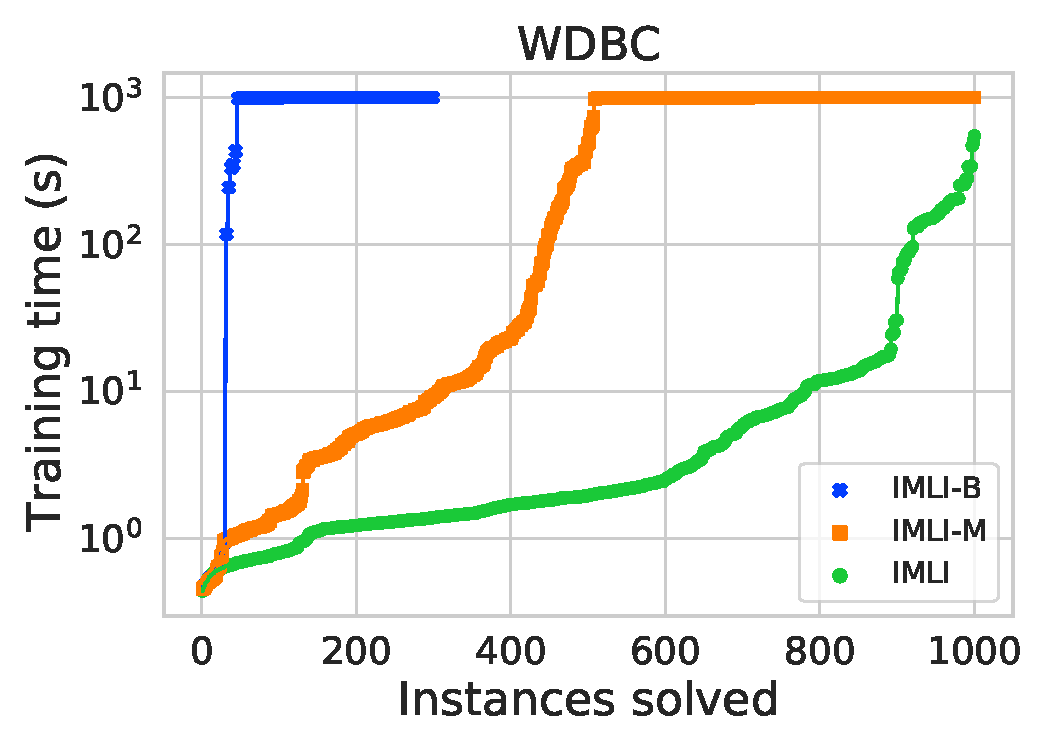
\includegraphics[scale=0.3]{figures/interpretability/imli/imli_exp_wdbc_cactus_train_val_fit_time}}	
	\subfloat{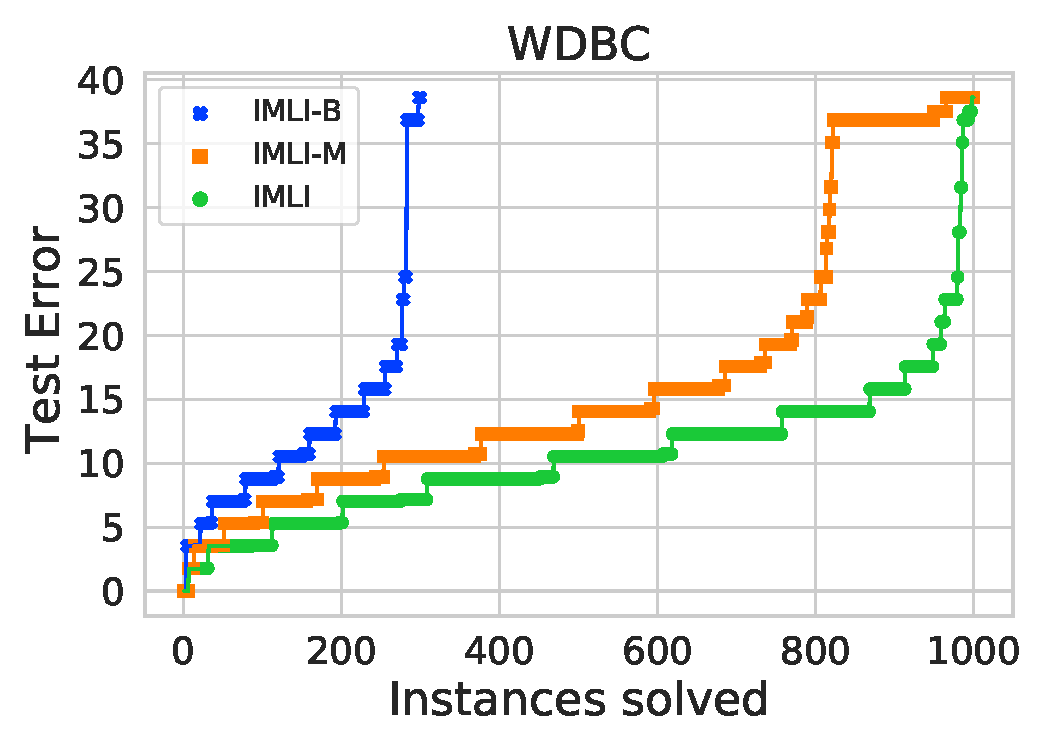
\includegraphics[scale=0.3]{figures/interpretability/imli/imli_exp_wdbc_cactus_test_accuracy}}
	\subfloat{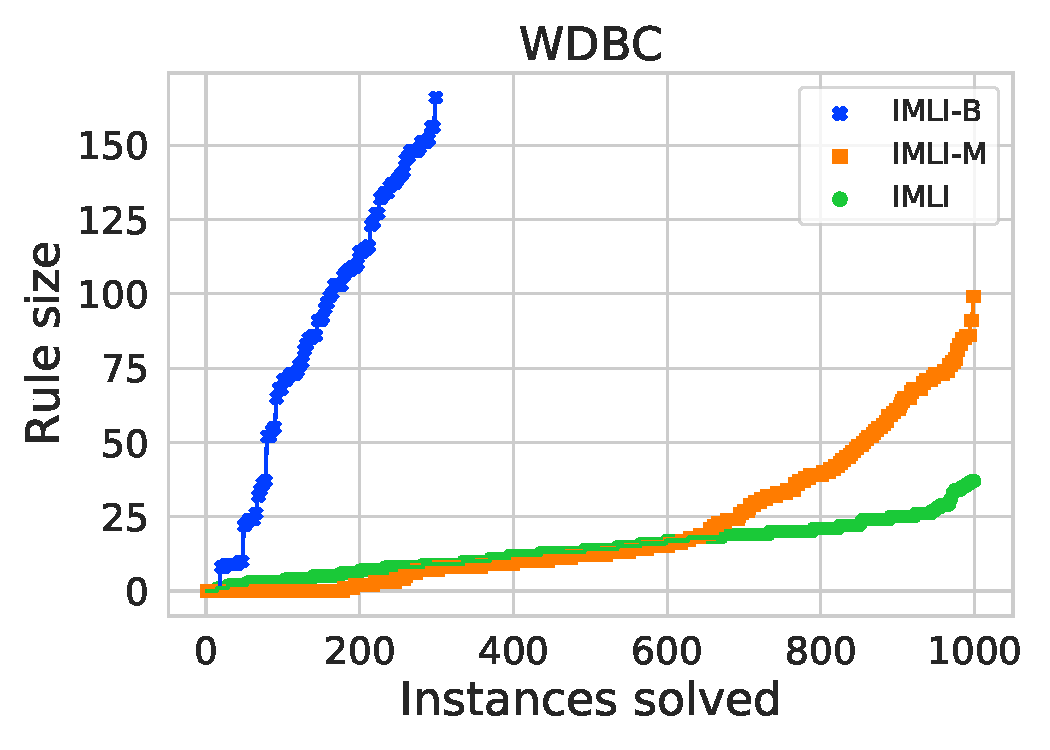
\includegraphics[scale=0.3]{figures/interpretability/imli/imli_exp_wdbc_cactus_predicate_count}}
		
	
	\subfloat{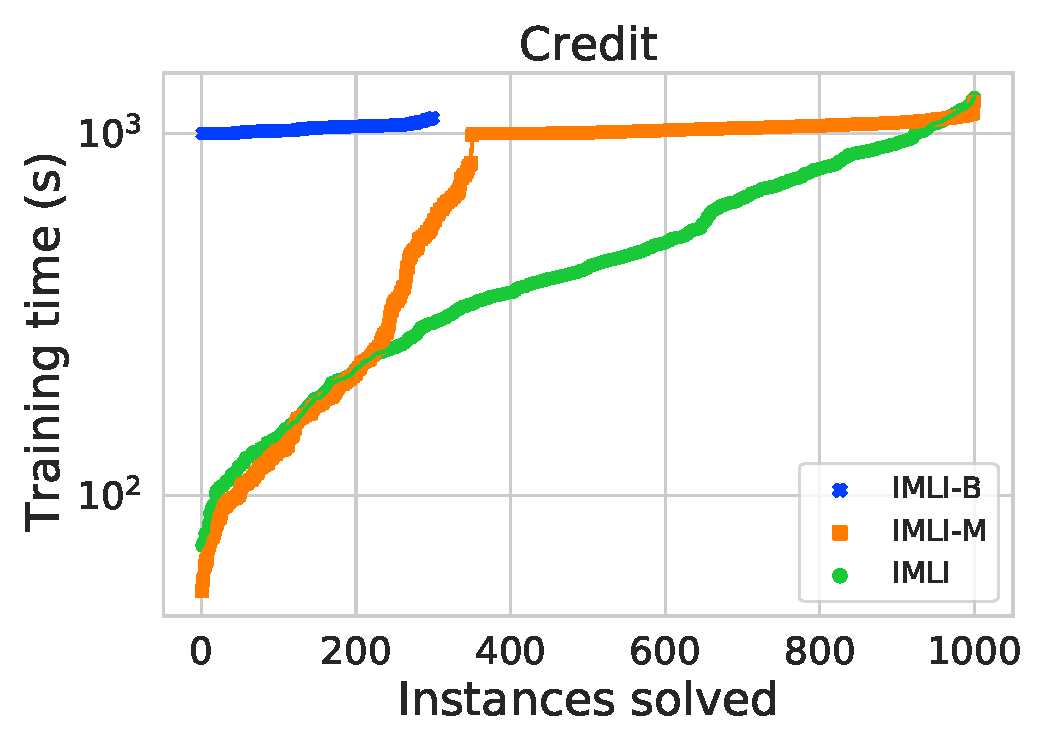
\includegraphics[scale=0.3]{figures/interpretability/imli/imli_exp_credit_cactus_train_val_fit_time}}	
	\subfloat{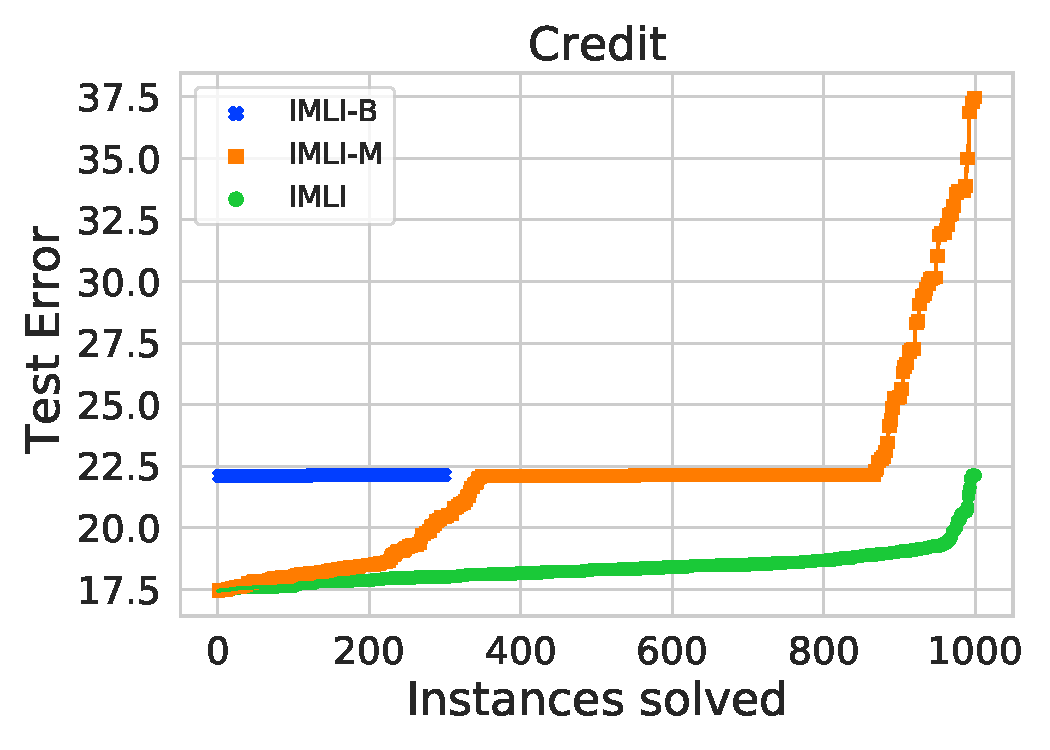
\includegraphics[scale=0.3]{figures/interpretability/imli/imli_exp_credit_cactus_test_accuracy}}
	\subfloat{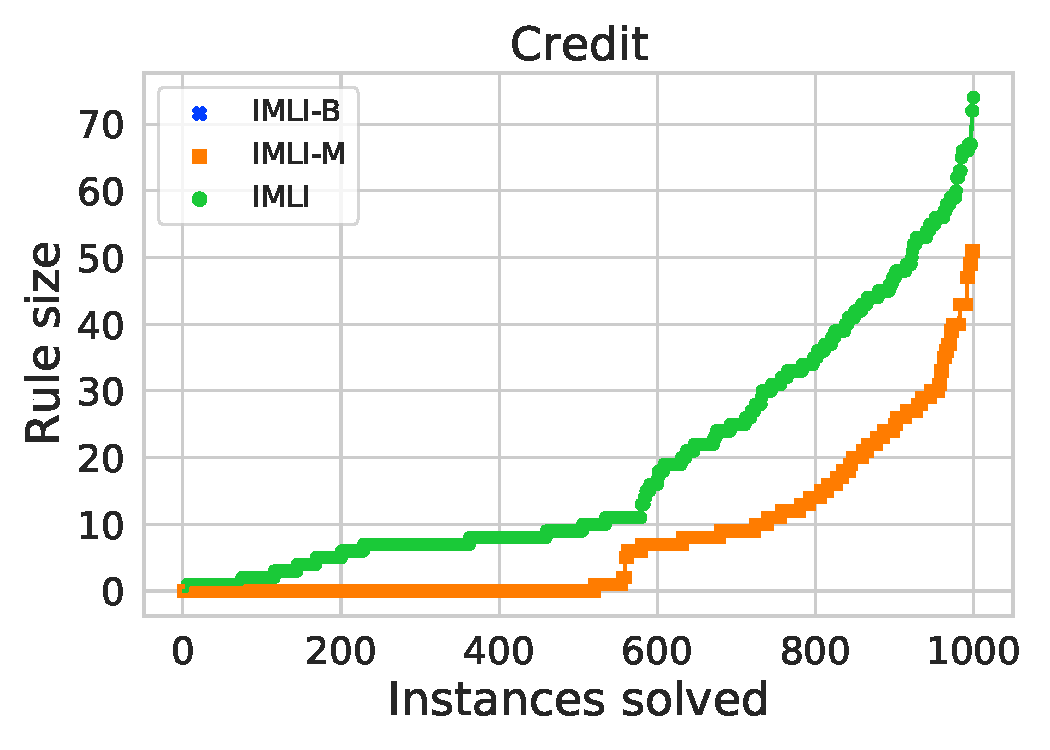
\includegraphics[scale=0.3]{figures/interpretability/imli/imli_exp_credit_cactus_predicate_count}}
	

	\subfloat{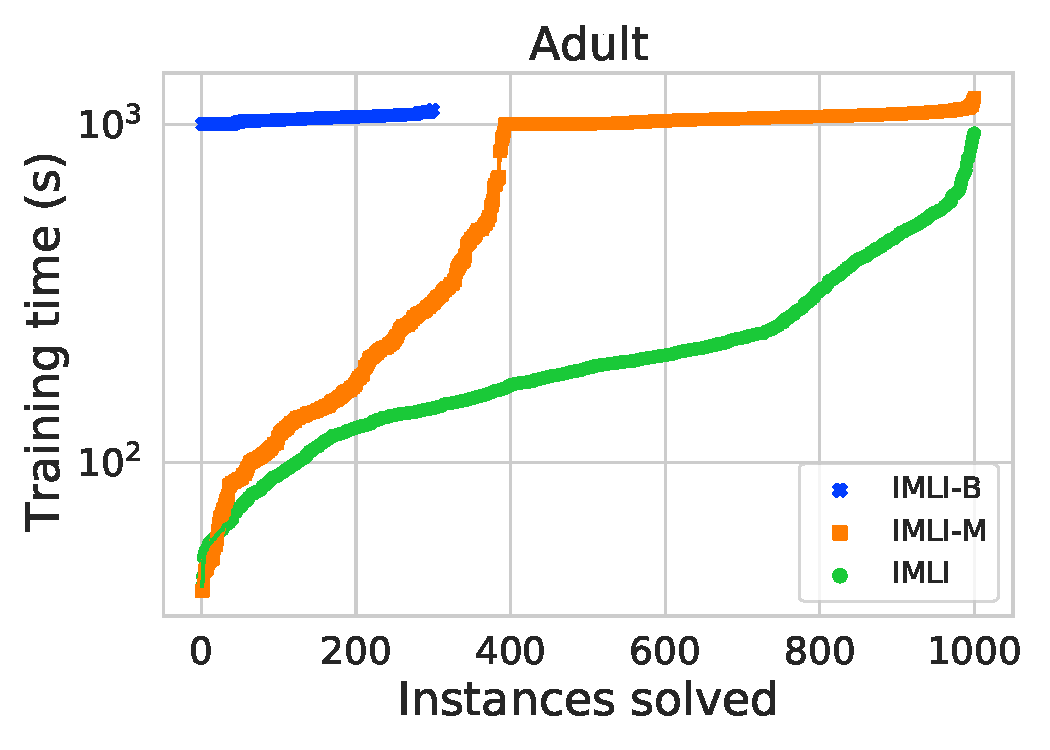
\includegraphics[scale=0.3]{figures/interpretability/imli/imli_exp_adult_cactus_train_val_fit_time}}	
	\subfloat{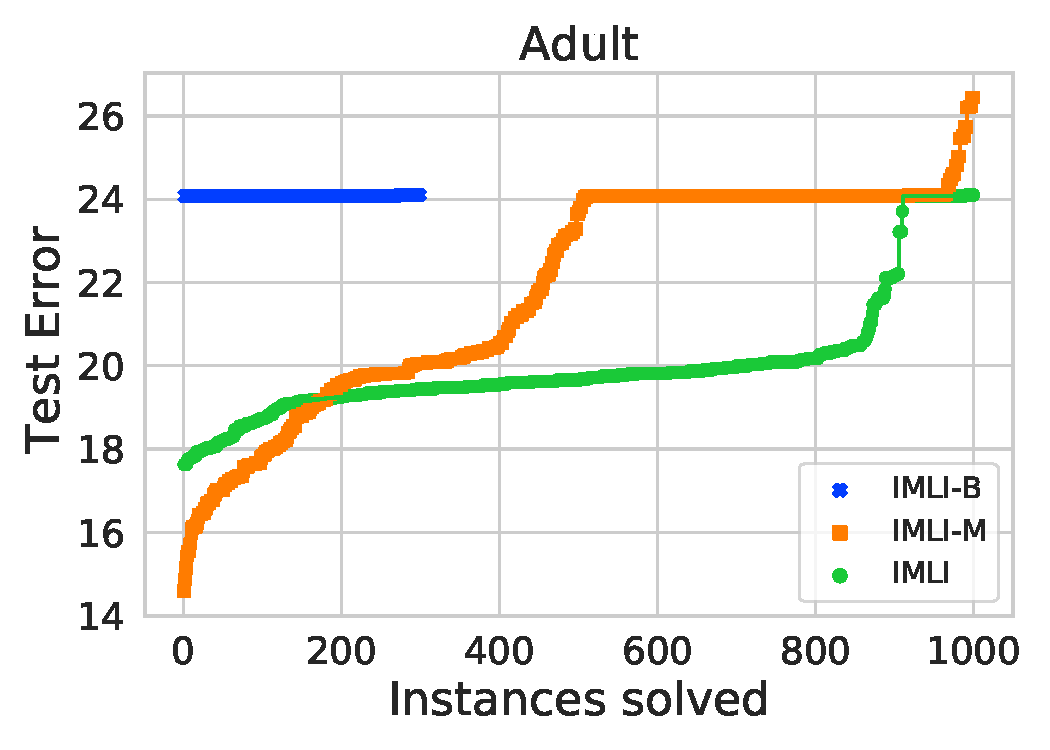
\includegraphics[scale=0.3]{figures/interpretability/imli/imli_exp_adult_cactus_test_accuracy}}
	\subfloat{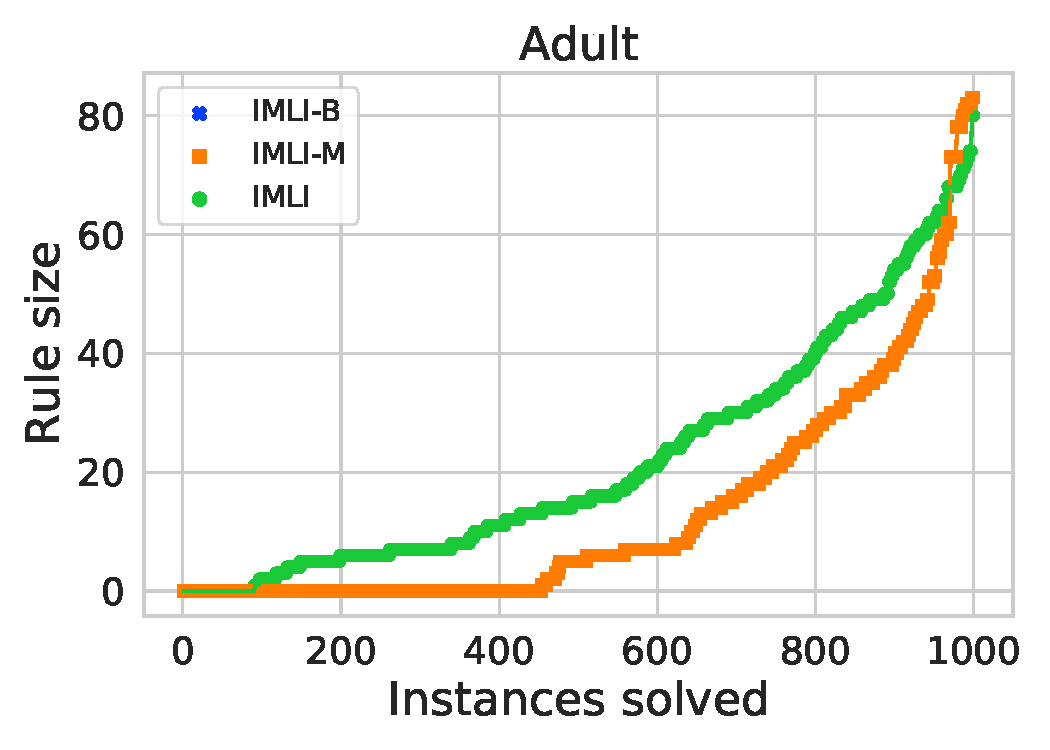
\includegraphics[scale=0.3]{figures/interpretability/imli/imli_exp_adult_cactus_predicate_count}}

	
	\caption[Training time, test error, and rule-size of different formulations in {\imli}]{Comparison of training time, test error, and rule-size among different formulations presented in the paper. In each cactus plot, the incremental formulation {\imli} with both mini-batch and iterative learning demonstrates the best performance in training time and test error than compared two formulations: non-incremental MaxSAT formulation {\imli}-$\mathsf{B}$ and incremental formulation with only mini-batch learning {\imli}-$\mathsf{M}$. In terms of rule-size, {\imli} often generates higher size rules than {\imli}-$\mathsf{M}$.}
	\label{interpretability_imli_fig:different_formulations}
\end{figure}



\paragraph{Comparison among different formulations in {\imli}.}  We compare the performance of different formulations for learning classification rules as presented in this paper. In Figure~\ref{interpretability_imli_fig:different_formulations}, we show cactus plots for assessing training time (in seconds), test error (in percentage), and rule-size among different formulations. In the cactus plot, a point $ (x,y) $ denotes that the formulation yields lower than or equal to $ y $ training time (similarly, test error and rule-size) in $ x $ many instances in each dataset.

In Figure~\ref{interpretability_imli_fig:different_formulations}, we denote the baseline non-incremental MaxSAT-based formulation as {\imli}-$\mathsf{B}$\footnote{Since  {\imli}-$\mathsf{B}$ is a non-incremental formulation and does not involve any mini-batch learning, we consider two hyper-parameters for {\imli}-$\mathsf{B}$: the number of clauses in $ \{1, 2, \dots, 10\} $ and the regularization parameter $ \lambda $ as $ 10 $ values chosen from a logarithmic grid between $ 10^{-4} $ and $ 10^1 $.}, incremental MaxSAT-based formulation with only mini-batch learning as {\imli}-$\mathsf{M}$, and incremental MaxSAT-based formulation with both mini-batch and iterative learning as {\imli}.  We first observe the training time of different formulations in the left-most column in Figure~\ref{interpretability_imli_fig:different_formulations}, where {\imli}-$\mathsf{B}$ soon times out and solves lower than $ 300 $ instances out of $ 1000 $ instances in each dataset. This result suggests that the non-incremental formulation cannot scale in practical classification task. Comparing between {\imli} and {\imli}-$\mathsf{M}$, both formulations solve all $ 1000 $ instances in each dataset with {\imli}-$\mathsf{M}$ undertaking significantly higher training time than $ {\imli} $.  Therefore, {\imli} achieves better scalability than {\imli}-$\mathsf{M}$ indicating that an integration of mini-batch and iterative learning achieves a significant progress in terms of scalability than mini-batch learning alone. 

We next focus on the test error of different formulations in the middle column in Figure~\ref{interpretability_imli_fig:different_formulations}. Firstly, {\imli}-$\mathsf{B}$ has a higher test error than the other two formulations since {\imli}-$\mathsf{B}$ times out in most instances and learns a sub-optimal classification rule with reduced prediction accuracy. In contrast, {\imli} has the lowest test error compared to two formulations in all datasets. This result indicates the effectiveness of integrating both iterative and mini-batch learning with MaxSAT-based formulation in generating more accurate classification rules.


Moving focus on the rule-size in the rightmost column in Figure~\ref{interpretability_imli_fig:different_formulations}, {\imli}-$\mathsf{B}$ achieves the highest rule-size in WDBC dataset. In contrast, the rule-size of {\imli}-$\mathsf{B}$  is lowest (zero) in Credit and Adult datasets. In the last two datasets, {\imli}-$\mathsf{B}$ times out during training and returns the default rule ``true'' by predicting all samples as class $ 1 $. The other two formulations {\imli} and {\imli}-$\mathsf{M}$  demonstrate a similar trend in rule-size in all datasets with {\imli}-$\mathsf{M}$ generating comparatively smaller size rules in Credit and Adult datasets. In this context,  the improvement of rule-sparsity of {\imli}-$\mathsf{M}$ is due to a comparatively higher test error (or lower accuracy) than {\imli} as observed in all three datasets. Therefore, {\imli} appears to be the best performing formulation w.r.t.\ training time, test error, and rule-size by balancing between accuracy and rule-size while being more scalable.

\begin{table*}[!t]        
	\centering
	\caption[Accuracy and rule-size of different classification rules learned using {\imli}]{Comparison of test accuracy (top value) and rule-size (bottom value) among different rule-based representations learned using {\imli}. Numbers in bold denote the best performing results among different representations.}
	\label{interpretability_imli_table:different_representations}
	%	\setlength{\tabcolsep}{.2em}
	\small
	\begin{tabular}{lrrrrrrrrrrrrrrr}
		
		
		
		


\toprule
Dataset & CNF & DNF & Decision Sets & Decision Lists \\

\midrule
\multirow{2}{*}{Parkinsons}  &
$ 94.74 $  &  $ 89.47 $  &  $ \mathbf{94.87} $  &  $ 89.74 $  \\
& $ 7.5 $  &  $ \mathbf{6.0} $  &  $ 15.0 $  &  $ 6.5 $  \\
\addlinespace[0.5em]

\multirow{2}{*}{WDBC}  &
$ 94.74 $  &  $ \mathbf{96.49} $  &  $ 95.61 $  &  $ 95.61 $  \\
& $ 11.5 $  &  $ 15.0 $  &  $ 15.5 $  &  $ \mathbf{10.0} $  \\
\addlinespace[0.5em]

\multirow{2}{*}{Pima}  &
$ \mathbf{78.43} $  &  $ 77.13 $  &  $ 76.97 $  &  $ 76.97 $  \\
& $ 23.0 $  &  $ \mathbf{9.0} $  &  $ 15.0 $  &  $ 13.5 $  \\
\addlinespace[0.5em]

\multirow{2}{*}{Titanic}  &
$ 81.82 $  &  $ 82.29 $  &  $ 81.82 $  &  $ \mathbf{82.3} $  \\
& $ \mathbf{5.5} $  &  $ 10.5 $  &  $ 8.5 $  &  $ 8.0 $  \\
\addlinespace[0.5em]

\multirow{2}{*}{MAGIC}  &
$ \mathbf{78.26} $  &  $ 77.44 $  &  $ 75.87 $  &  $ 77.79 $  \\
& $ \mathbf{8.5} $  &  $ 41.5 $  &  $ 10.0 $  &  $ 14.0 $  \\
\addlinespace[0.5em]

\multirow{2}{*}{Tom's HW}  &
$ 85.24 $  &  $ 85.15 $  &  $ 85.72 $  &  $ \mathbf{85.95} $  \\
& $ 44.5 $  &  $ \mathbf{26.5} $  &  $ 45.0 $  &  $ 59.5 $  \\
\addlinespace[0.5em]

\multirow{2}{*}{Credit}  &
$ 82.12 $  &  $ 82.15 $  &  $ 82.03 $  &  $ \mathbf{82.22} $  \\
& $ 17.5 $  &  $ 14.0 $  &  $ \mathbf{9.5} $  &  $ 21.5 $  \\
\addlinespace[0.5em]

\multirow{2}{*}{Adult}  &
$ 81.2 $  &  $ \mathbf{84.28} $  &  $ 80.07 $  &  $ 80.96 $  \\
& $ 30.0 $  &  $ 34.5 $  &  $ \mathbf{7.0} $  &  $ 24.5 $  \\
\addlinespace[0.5em]

\multirow{2}{*}{Bank Marketing}  &
$ \mathbf{89.84} $  &  $ 89.77 $  &  $ 89.67 $  &  $ 89.79 $  \\
& $ 24.5 $  &  $ 7.5 $  &  $ \mathbf{6.0} $  &  $ 10.5 $  \\
\addlinespace[0.5em]

\multirow{2}{*}{Connect-4}  &
$ \mathbf{75.36} $  &  $ 70.63 $  &  $ 68.09 $  &  $ 69.83 $  \\
& $ 50.5 $  &  $ 42.0 $  &  $ \mathbf{4.5} $  &  $ 24.0 $  \\
\addlinespace[0.5em]

\multirow{2}{*}{Weather AUS}  &
$ 83.78 $  &  $ \mathbf{84.23} $  &  $ 83.69 $  &  $ 83.85 $  \\
& $ 22.0 $  &  $ 14.0 $  &  $ \mathbf{4.0} $  &  $ 26.0 $  \\
\addlinespace[0.5em]


\multirow{2}{*}{Skin Seg}  &
$ \mathbf{94.71} $  &  $ 93.68 $  &  $ 87.92 $  &  $ 91.17 $  \\
& $ 30.0 $  &  $ 15.0 $  &  $ \mathbf{3.0} $  &  $ 7.0 $  \\
\bottomrule

	
				
	\end{tabular}
	
\end{table*}




\paragraph{Performance evaluation of different interpretable representations in {\imli}.}

We deploy {\imli} to learn different interpretable rule-based representations: CNF and DNF classifiers, decision lists, and decision sets and present their comparative performance w.r.t.\ test accuracy and rule-size in Table~\ref{interpretability_imli_table:different_representations}. In each cell in this table, the top value represents the test accuracy and the bottom value represents the size of generated rules.


We learn all four interpretable representations on twelve datasets, where the CNF classifier appears to be the most accurate representation by achieving the highest accuracy in five datasets. In contrast, both DNF and decision lists achieve the highest accuracy in three datasets each; decision sets demonstrate the least performance in test accuracy by being more accurate in one dataset. To this end, the poor accuracy of decision sets is traded off by its rule-size as decision sets generate the sparsest rules compared to other representations. More precisely, decision sets have the smallest rule-size in six datasets, while CNF, DNF, and decision lists have the smallest rule-size in two, three, and one dataset, respectively. These results suggest that CNF classifiers are more favored in applications where higher accuracy is preferred, while decision sets are preferred in applications where higher interpretability is desired. In both cases, one could deploy {\imli} for learning varied representations of classification rules. 




\begin{figure}[!t]
	
	\centering
	
	\subfloat{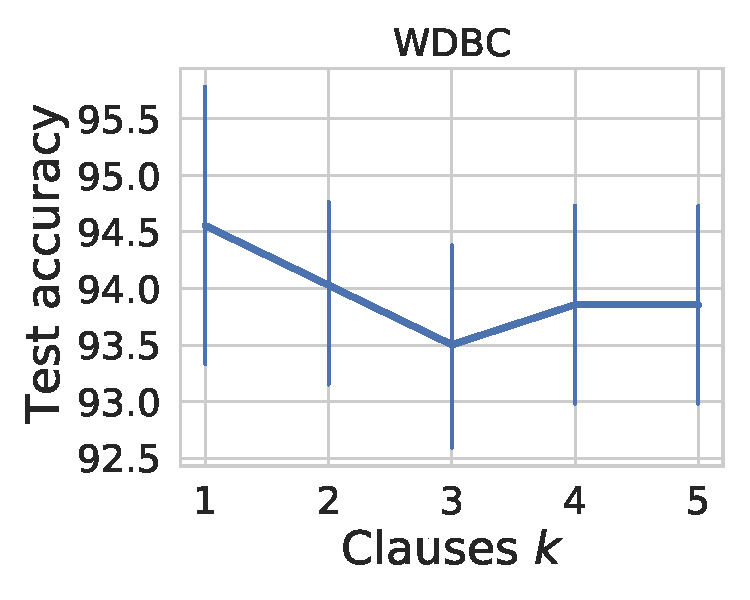
\includegraphics[scale=0.3]{figures/interpretability/imli/clauses_test_accuracy_wdbc}}
	\subfloat{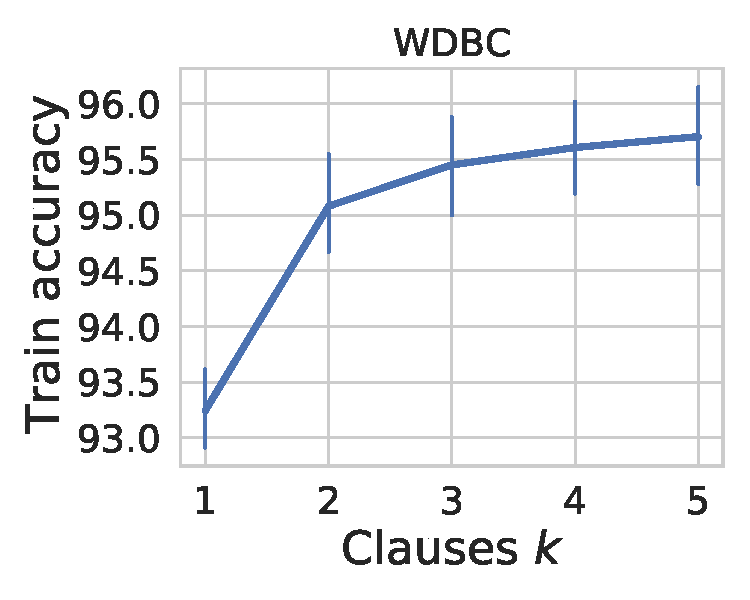
\includegraphics[scale=0.3]{figures/interpretability/imli/clauses_train_val_accuracy_wdbc}}
	\subfloat{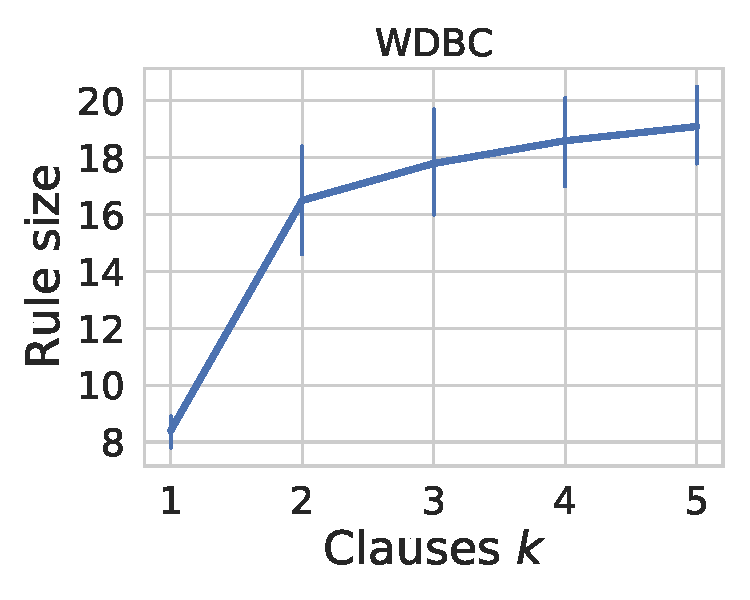
\includegraphics[scale=0.3]{figures/interpretability/imli/clauses_predicate_count_wdbc}}
	\subfloat{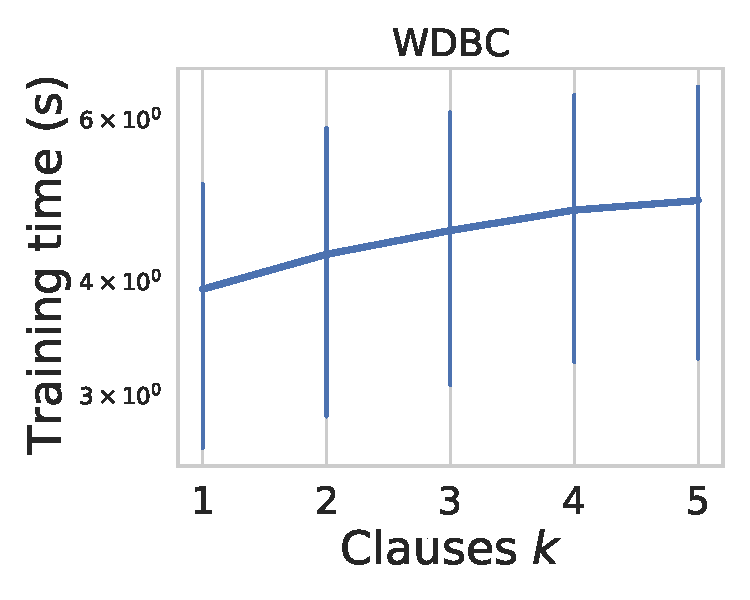
\includegraphics[scale=0.3]{figures/interpretability/imli/clauses_train_val_fit_time_wdbc}}
	
	
	\subfloat{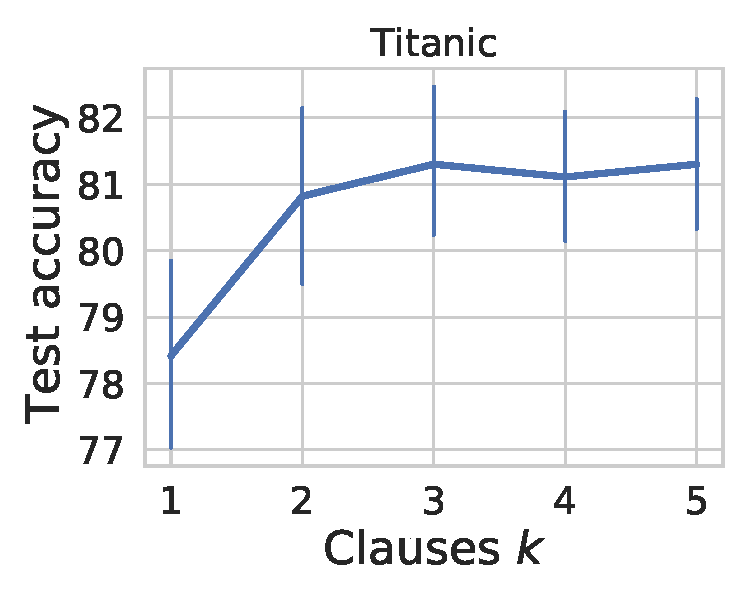
\includegraphics[scale=0.3]{figures/interpretability/imli/clauses_test_accuracy_titanic}}
	\subfloat{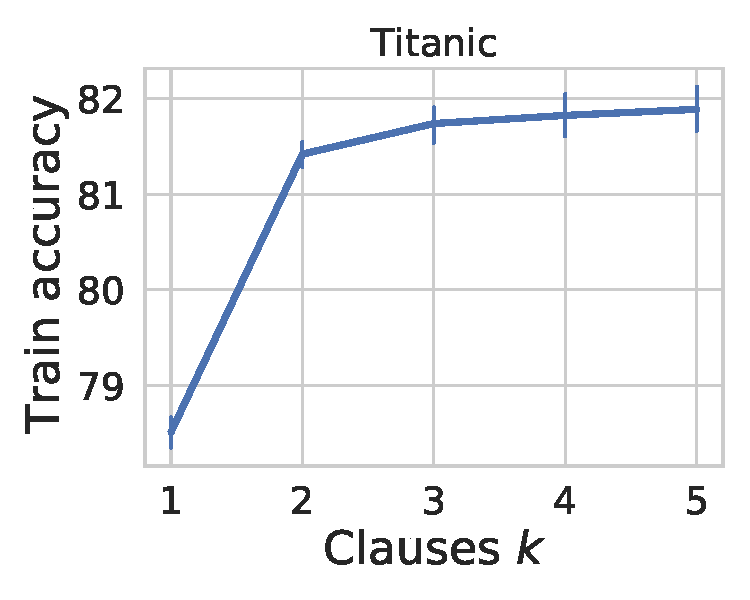
\includegraphics[scale=0.3]{figures/interpretability/imli/clauses_train_val_accuracy_titanic}}
	\subfloat{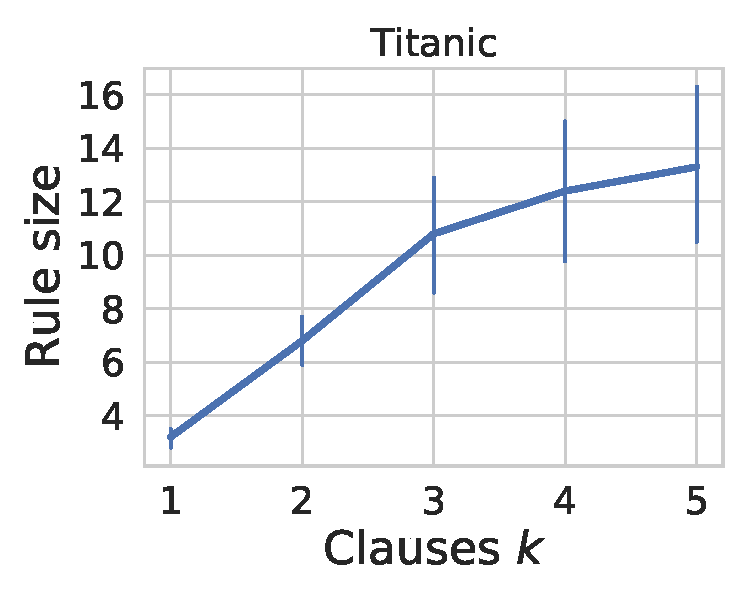
\includegraphics[scale=0.3]{figures/interpretability/imli/clauses_predicate_count_titanic}}
	\subfloat{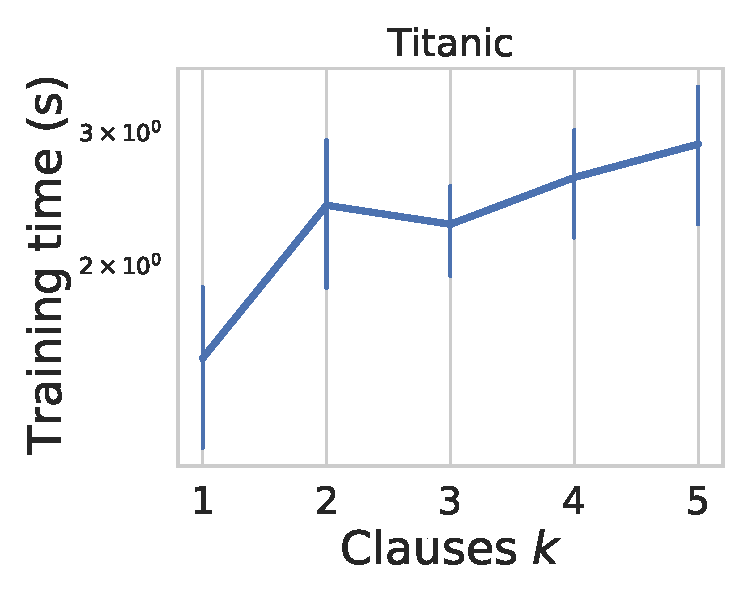
\includegraphics[scale=0.3]{figures/interpretability/imli/clauses_train_val_fit_time_titanic}}
	
	
	\subfloat{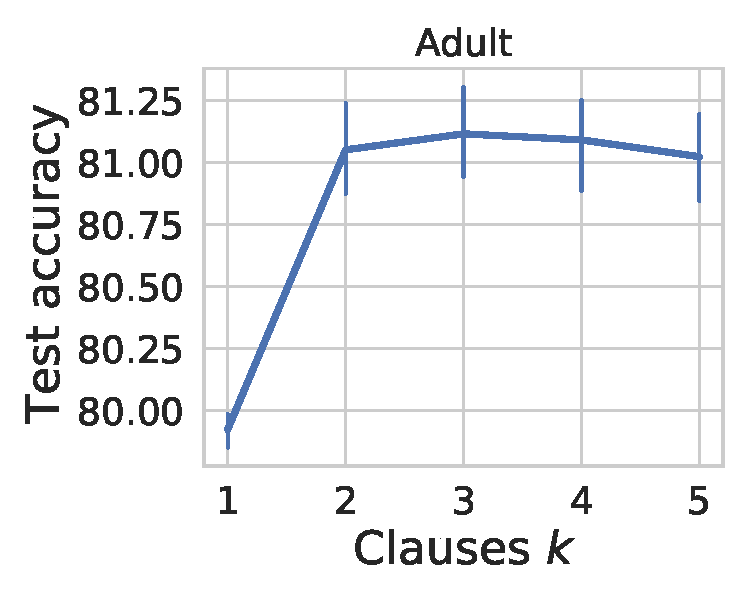
\includegraphics[scale=0.3]{figures/interpretability/imli/clauses_test_accuracy_adult}}
	\subfloat{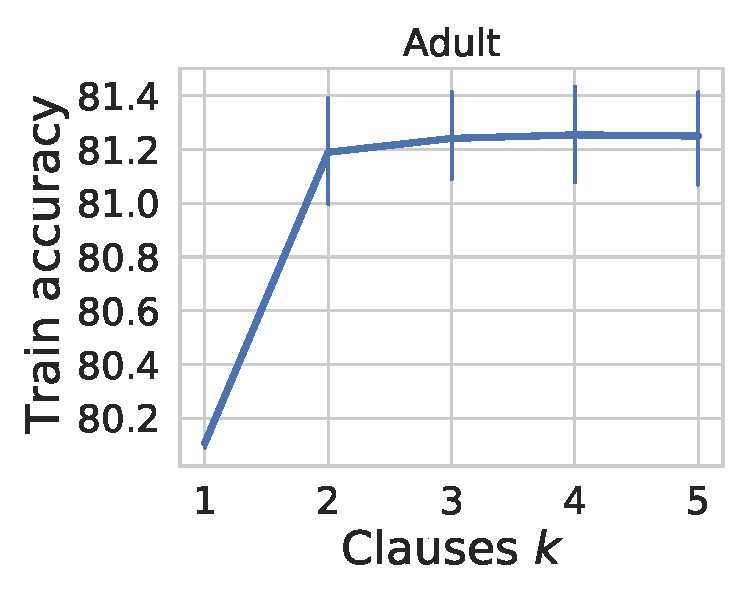
\includegraphics[scale=0.3]{figures/interpretability/imli/clauses_train_val_accuracy_adult}}
	\subfloat{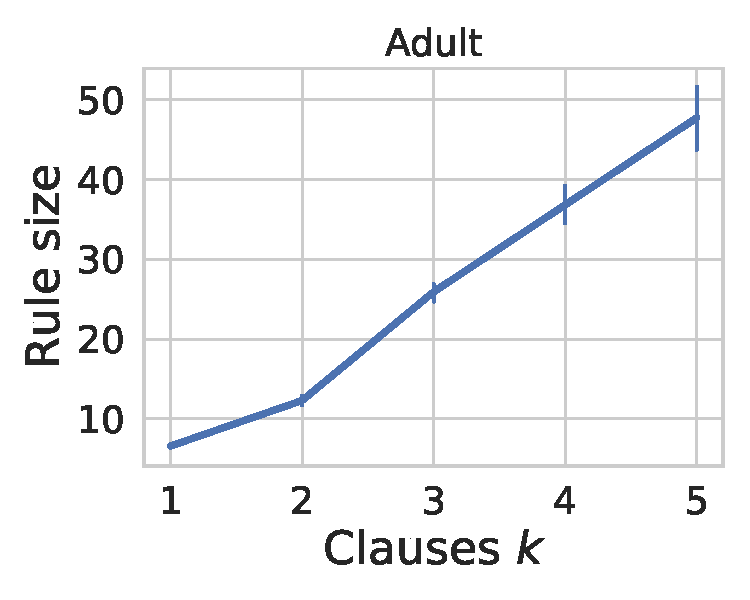
\includegraphics[scale=0.3]{figures/interpretability/imli/clauses_predicate_count_adult}}
	\subfloat{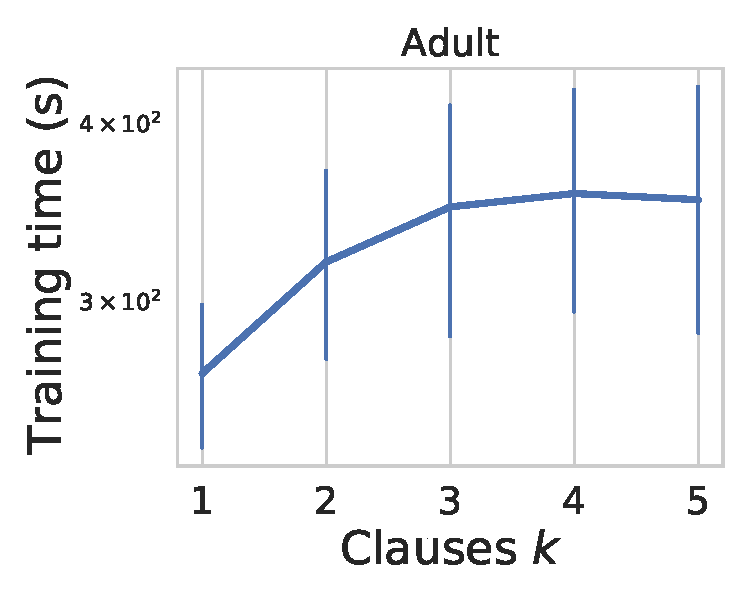
\includegraphics[scale=0.3]{figures/interpretability/imli/clauses_train_val_fit_time_adult}}
	
	
	
	
	\caption[Effect of the number of clauses in {\imli}]{Effect of the number of clauses $ k $ on accuracy (test and train), rule-size, and training time. As $ k $ increases, both train and test accuracy of {\imli} increase while generating rules with higher size by incurring higher training time. }
	\label{interpretability_imli_fig:effect_of_number_of_clauses}
\end{figure}

\paragraph{Ablation study.} We experiment the effect of different hyper-parameters in {\imli} on prediction accuracy, rule-size, and training time in different datasets. In the following, we discuss the impact of the number of clauses, regularization parameter, and size of mini-batches in {\imli}.


\textbf{Effect of the number of clauses $ k $.} In Figure~\ref{interpretability_imli_fig:effect_of_number_of_clauses}, we vary  $ k $ while learning CNF classifiers in {\imli}. As $ k $ increases, both training and test accuracy generally increase in different datasets (plots in the first and second columns). Similarly, the size of rules increases with $ k $ by incurring higher training time (plots in the third and fourth columns). The reason is that a higher value of $ k $ allows more flexibility in fitting the data well by incurring more training time and generating higher size classification rules. Therefore, the number of clauses in {\imli} provides control on training-time vs accuracy and also on accuracy vs rule-sparsity. 


\textbf{Effect of regularizer $ \lambda $.} In Figure~\ref{interpretability_imli_fig:effect_of_number_of_regularization}, we vary $ \lambda $ in a logarithmic grid between $ 10^{-4} $ and $ 10^1 $. As stated in Eq.~\eqref{interpretability_imli_eq:obj_incr}, a higher value of $ \lambda $ puts more priority on the minimal changes in rules between consecutive mini-batches in incremental learning while allowing higher mini-batch errors. Thus, in the first and second columns in Figure~\ref{interpretability_imli_fig:effect_of_number_of_regularization}, as $ \lambda $ increases, both training and test accuracy gradually decrease. In addition, the size of rules (plots in the third column) also decreases. Finally, we observe that the training time generally decreases with $ \lambda $. This observation indicates that higher $ \lambda $ puts lower computational load to the MaxSAT solver as a fraction of training examples is allowed to be misclassified. Thus, similar to the number of clauses, regularization parameter $ \lambda $ in {\imli} allows to trade-off between accuracy and rule-size in a precise manner.

\textbf{Effect of the size of mini-batch.} In Figure~\ref{interpretability_imli_fig:effect_of_batch_size}, we present the effect of mini-batch size in {\imli}. As we consider more samples in a batch, both test and training accuracy increase in general as presented in the first and second columns in Figure~\ref{interpretability_imli_fig:effect_of_batch_size}. Similarly, the size of generated rules also increases with the number of samples. Due to solving higher size MaxSAT queries, the training time also increases in general with an increase in mini-batch size. Therefore, by varying the size of mini-batches, {\imli} allows controlling on training time vs the prediction accuracy (and rule-size) of generated rules. 


\begin{figure}[!t]
	
	\centering
	
	
	\subfloat{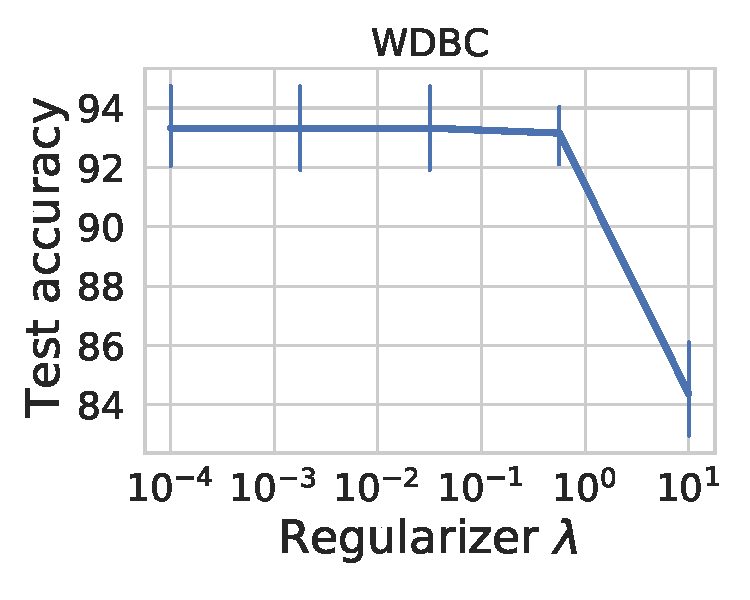
\includegraphics[scale=0.3]{figures/interpretability/imli/lambda__test_accuracy_wdbc}}
	\subfloat{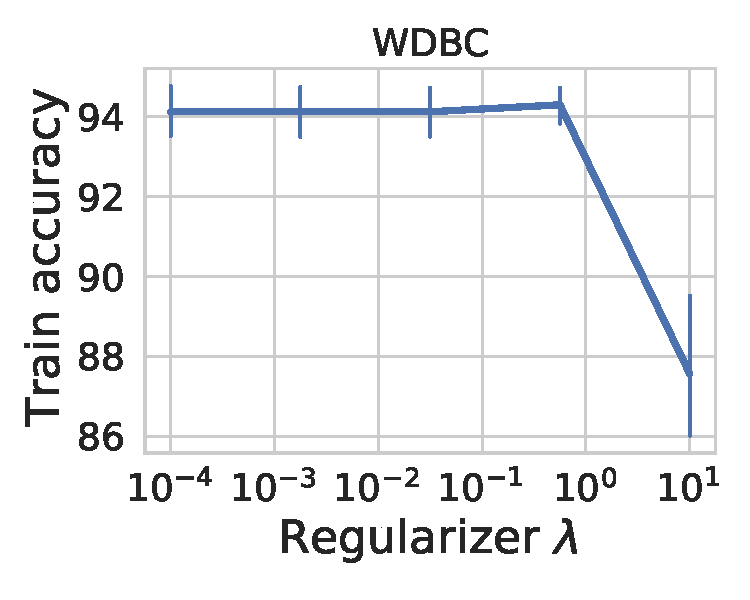
\includegraphics[scale=0.3]{figures/interpretability/imli/lambda__train_val_accuracy_wdbc}}
	\subfloat{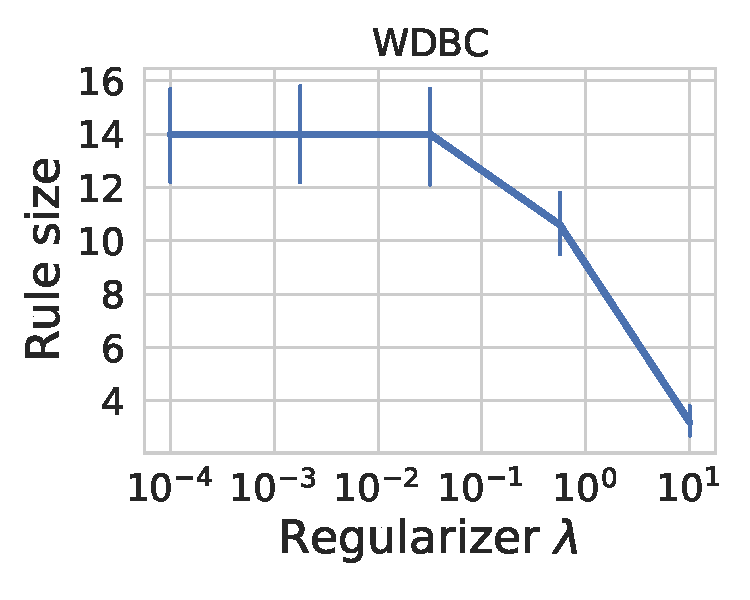
\includegraphics[scale=0.3]{figures/interpretability/imli/lambda__predicate_count_wdbc}}
	\subfloat{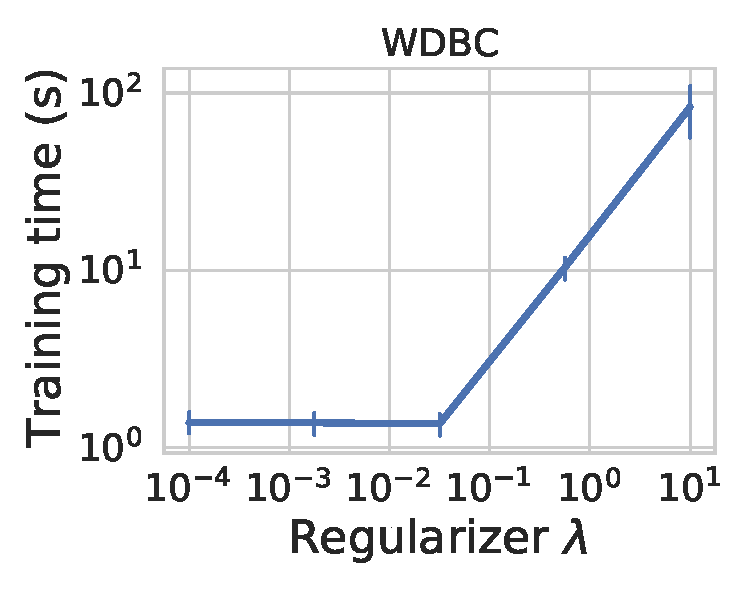
\includegraphics[scale=0.3]{figures/interpretability/imli/lambda__train_val_fit_time_wdbc}}


	\subfloat{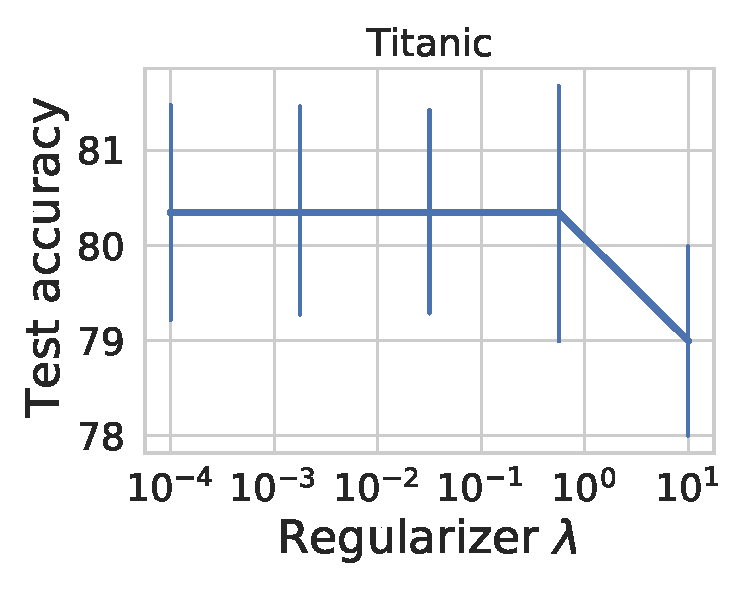
\includegraphics[scale=0.3]{figures/interpretability/imli/lambda__test_accuracy_titanic}}
	\subfloat{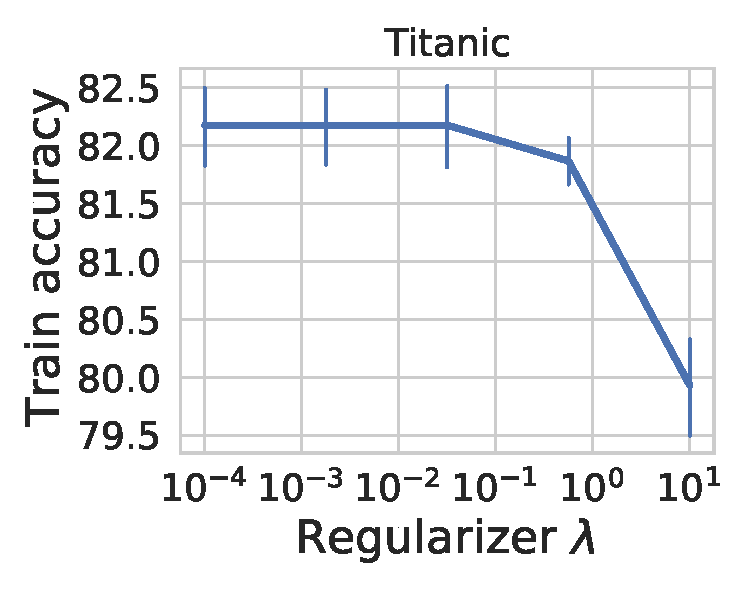
\includegraphics[scale=0.3]{figures/interpretability/imli/lambda__train_val_accuracy_titanic}}
	\subfloat{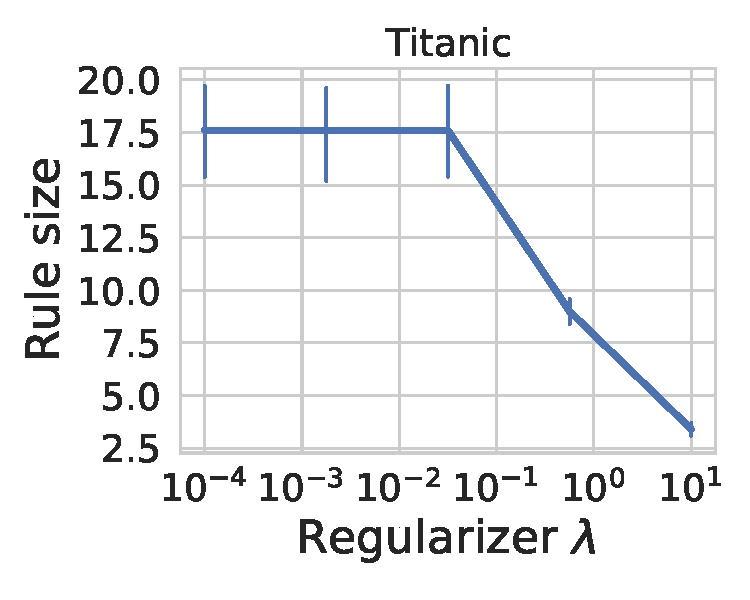
\includegraphics[scale=0.3]{figures/interpretability/imli/lambda__predicate_count_titanic}}
	\subfloat{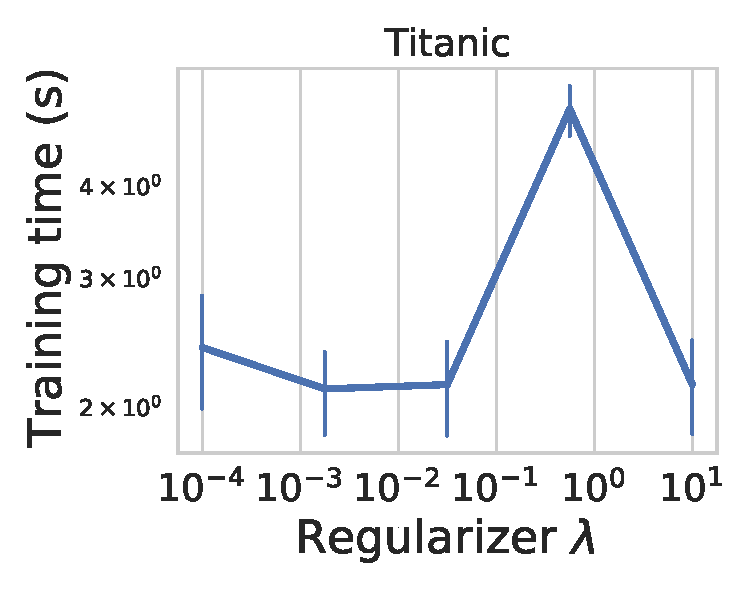
\includegraphics[scale=0.3]{figures/interpretability/imli/lambda__train_val_fit_time_titanic}}	
	
	\subfloat{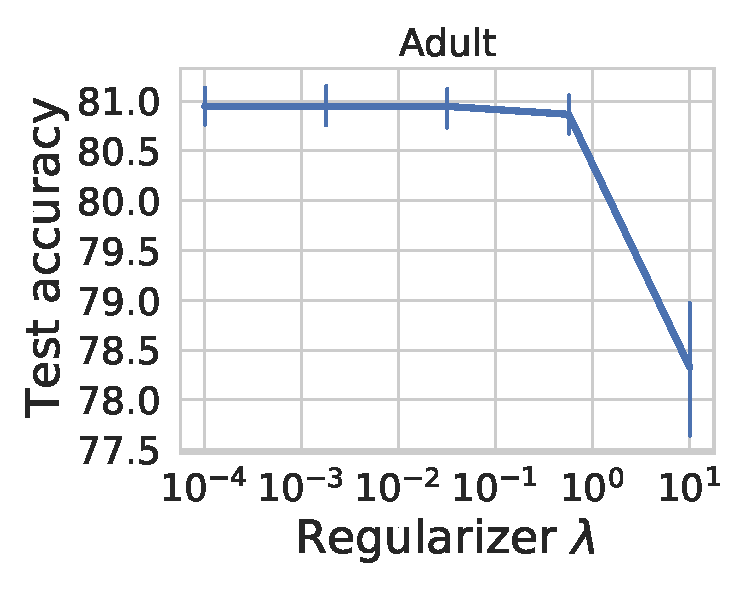
\includegraphics[scale=0.3]{figures/interpretability/imli/lambda__test_accuracy_adult}}
	\subfloat{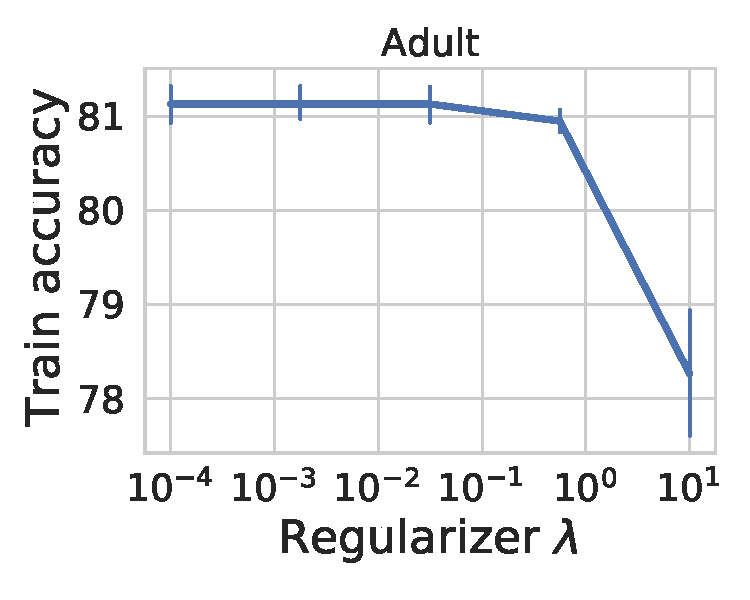
\includegraphics[scale=0.3]{figures/interpretability/imli/lambda__train_val_accuracy_adult}}
	\subfloat{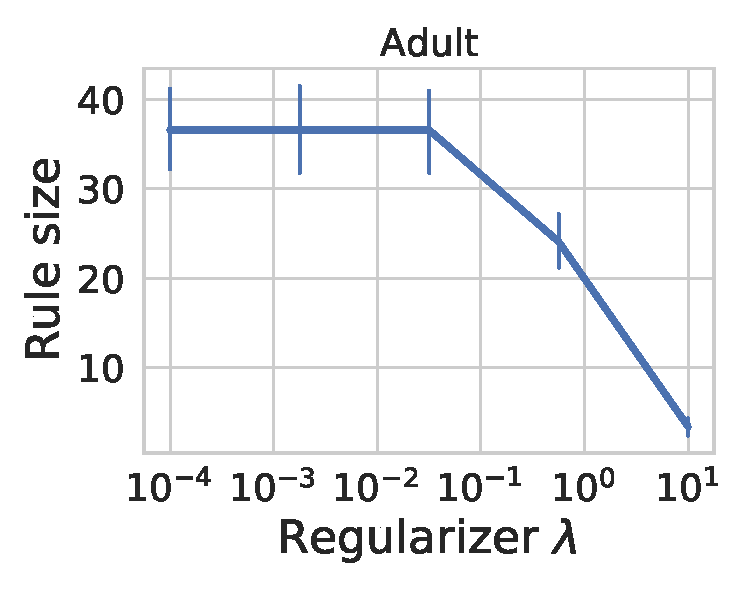
\includegraphics[scale=0.3]{figures/interpretability/imli/lambda__predicate_count_adult}}
	\subfloat{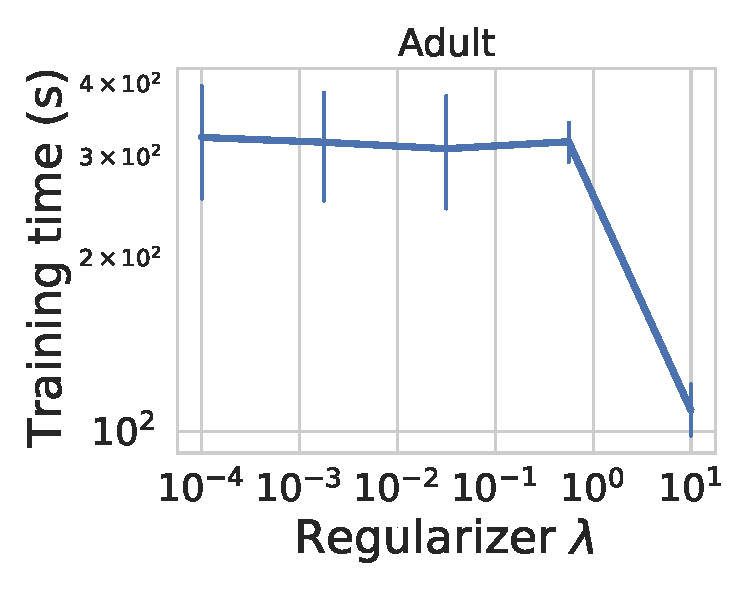
\includegraphics[scale=0.3]{figures/interpretability/imli/lambda__train_val_fit_time_adult}}
	
	
	
	
	
	\caption[Effect of regularization $ \lambda $ in {\imli}]{Effect of regularization $ \lambda $ on accuracy (test and train), rule-size, and training time. As $ \lambda $ increases, lower priority is given to accuracy. As a result, both training and test accuracy decrease with $ \lambda $ by generating smaller rules. }
	\label{interpretability_imli_fig:effect_of_number_of_regularization}
\end{figure}



\begin{figure}[!t]
	
	\centering
	
	\subfloat{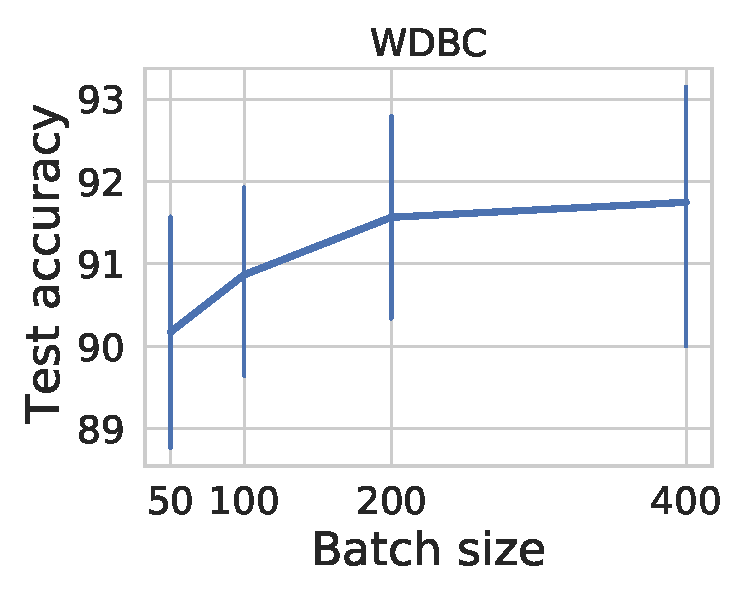
\includegraphics[scale=0.3]{figures/interpretability/imli/batch_size_test_accuracy_wdbc}}
	\subfloat{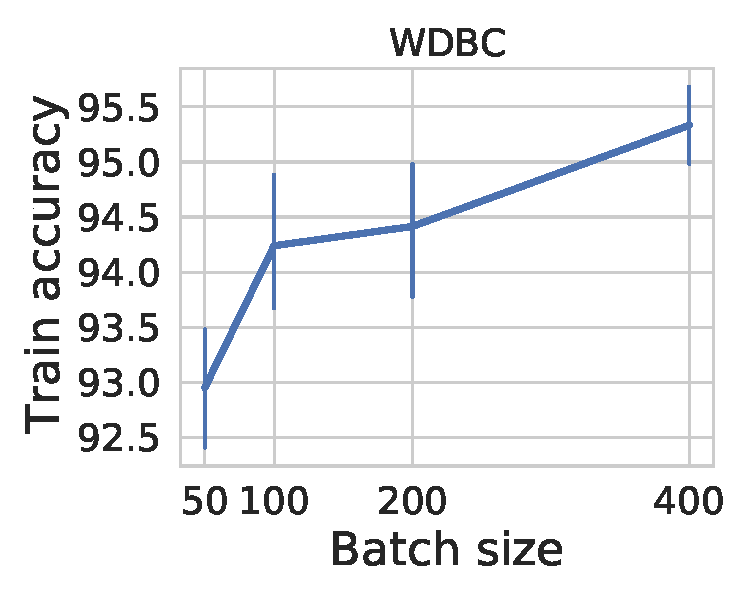
\includegraphics[scale=0.3]{figures/interpretability/imli/batch_size_train_val_accuracy_wdbc}}
	\subfloat{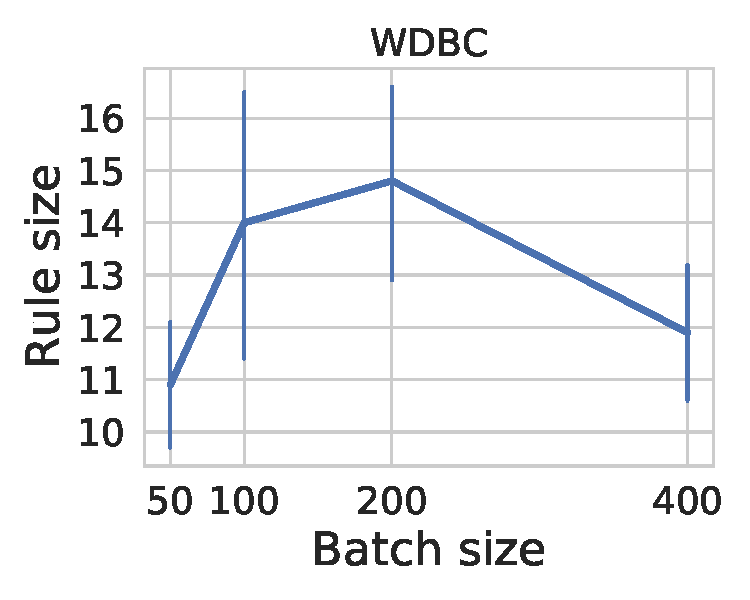
\includegraphics[scale=0.3]{figures/interpretability/imli/batch_size_predicate_count_wdbc}}
	\subfloat{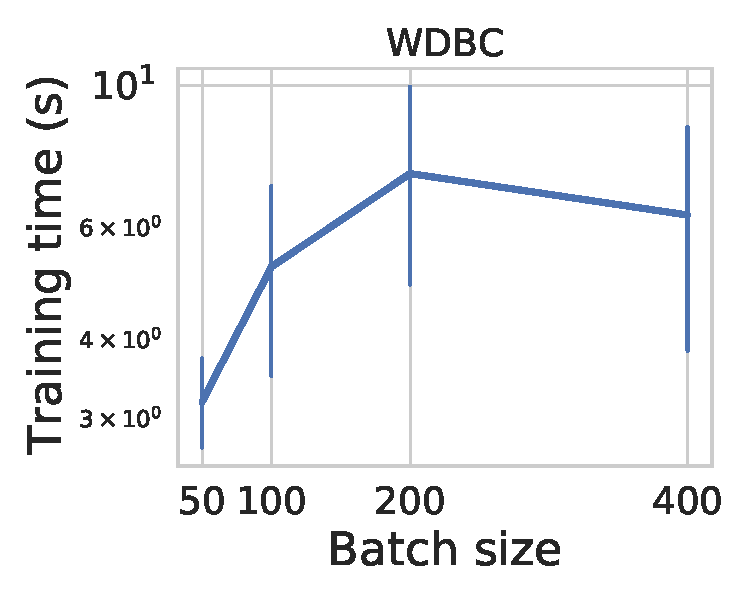
\includegraphics[scale=0.3]{figures/interpretability/imli/batch_size_train_val_fit_time_wdbc}}
	
	
	\subfloat{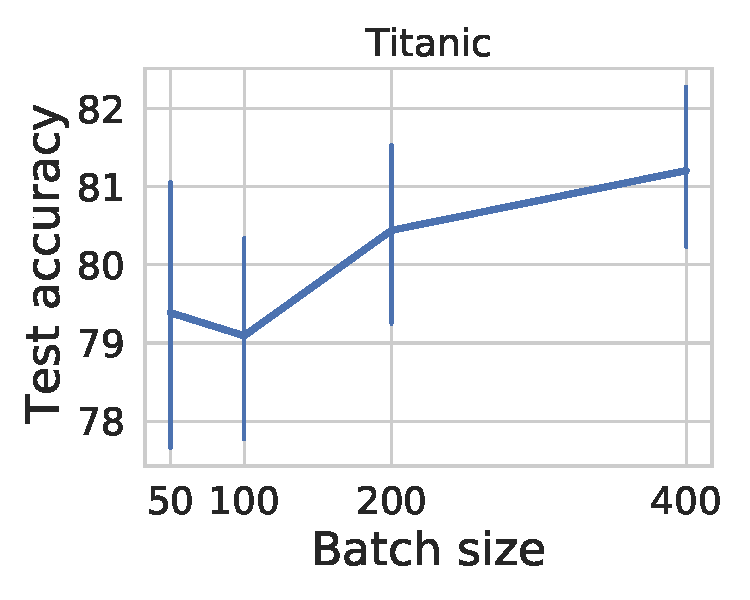
\includegraphics[scale=0.3]{figures/interpretability/imli/batch_size_test_accuracy_titanic}}
	\subfloat{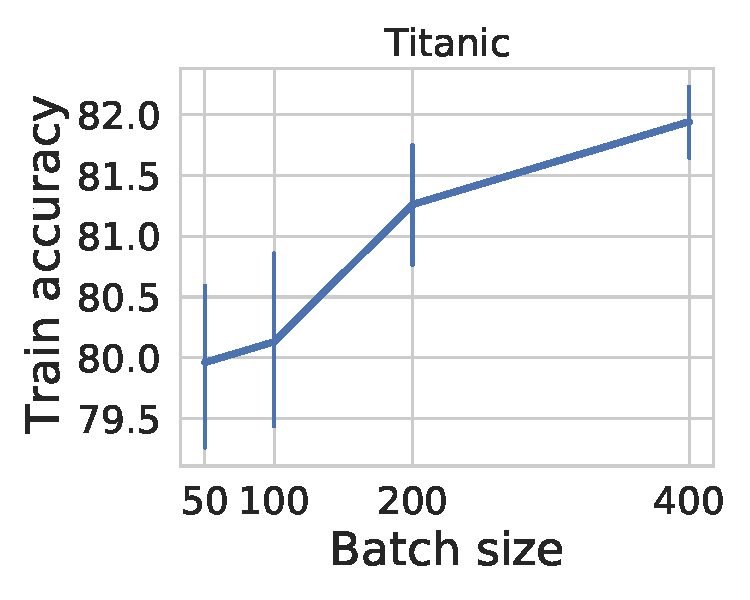
\includegraphics[scale=0.3]{figures/interpretability/imli/batch_size_train_val_accuracy_titanic}}
	\subfloat{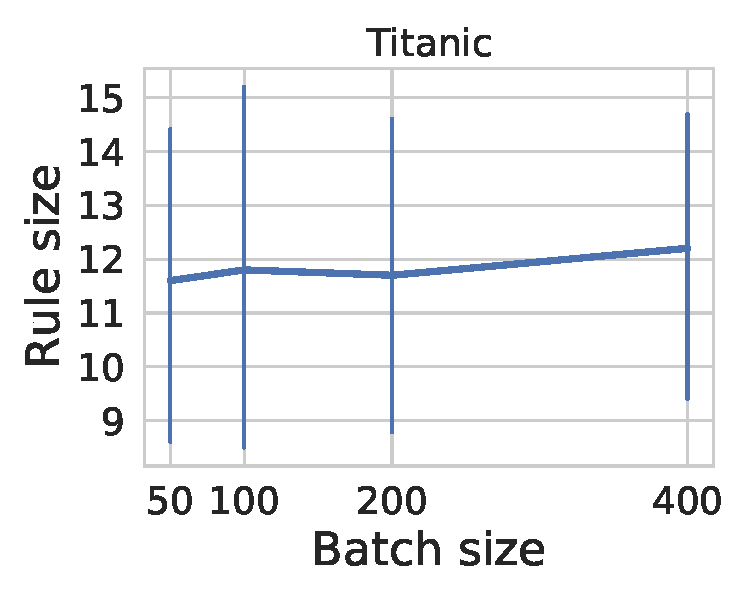
\includegraphics[scale=0.3]{figures/interpretability/imli/batch_size_predicate_count_titanic}}
	\subfloat{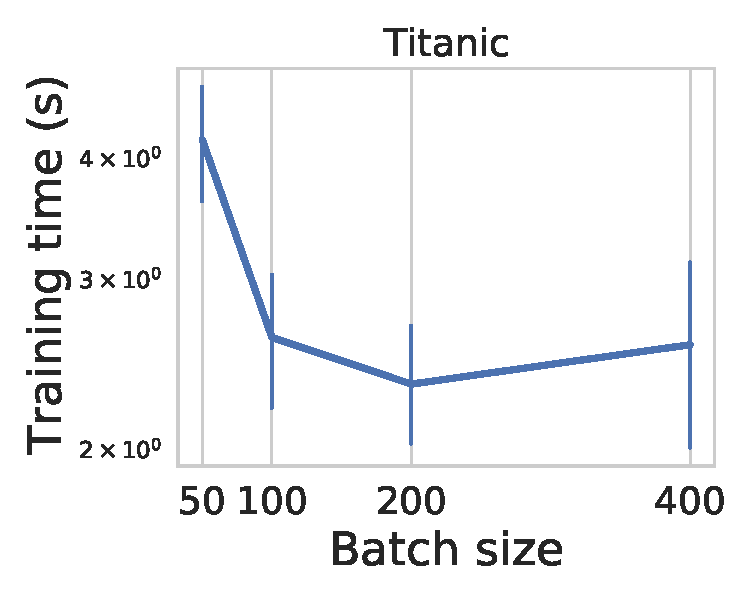
\includegraphics[scale=0.3]{figures/interpretability/imli/batch_size_train_val_fit_time_titanic}}	
	
	\subfloat{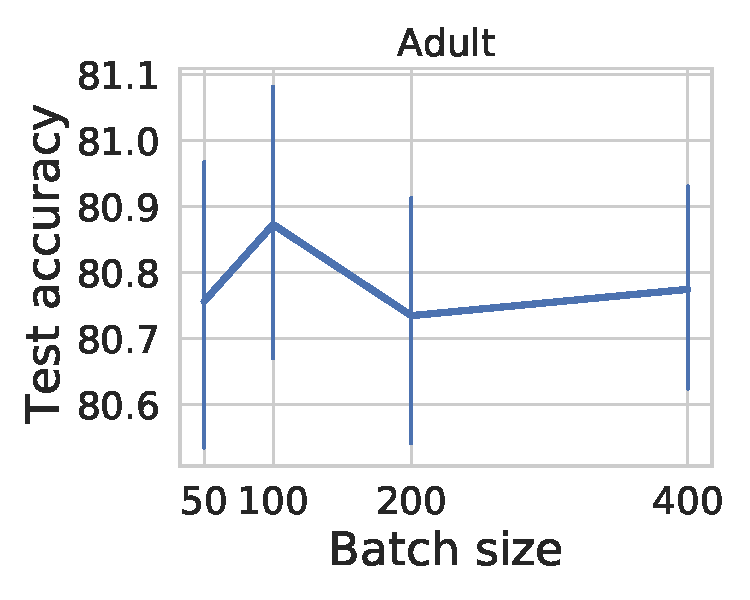
\includegraphics[scale=0.3]{figures/interpretability/imli/batch_size_test_accuracy_adult}}
	\subfloat{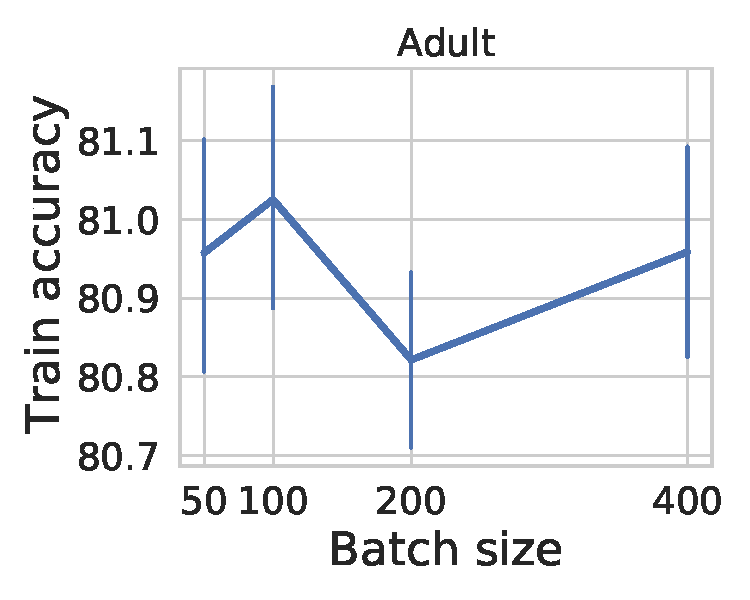
\includegraphics[scale=0.3]{figures/interpretability/imli/batch_size_train_val_accuracy_adult}}
	\subfloat{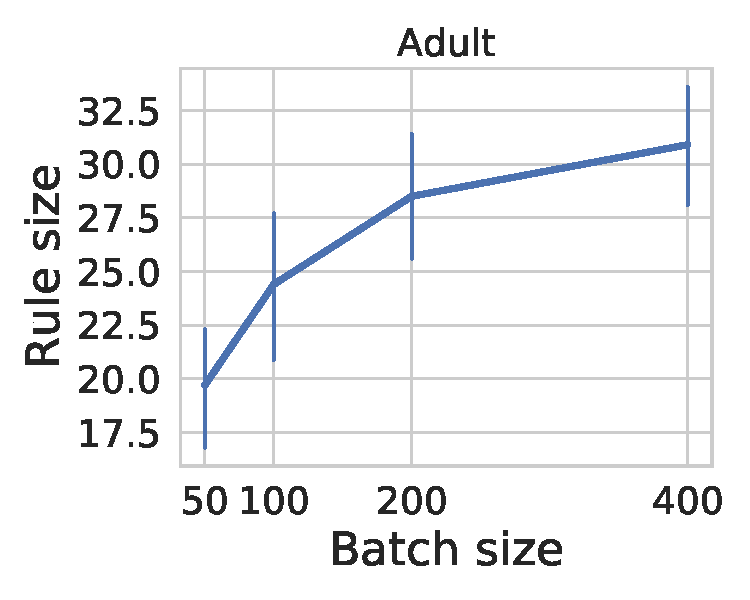
\includegraphics[scale=0.3]{figures/interpretability/imli/batch_size_predicate_count_adult}}
	\subfloat{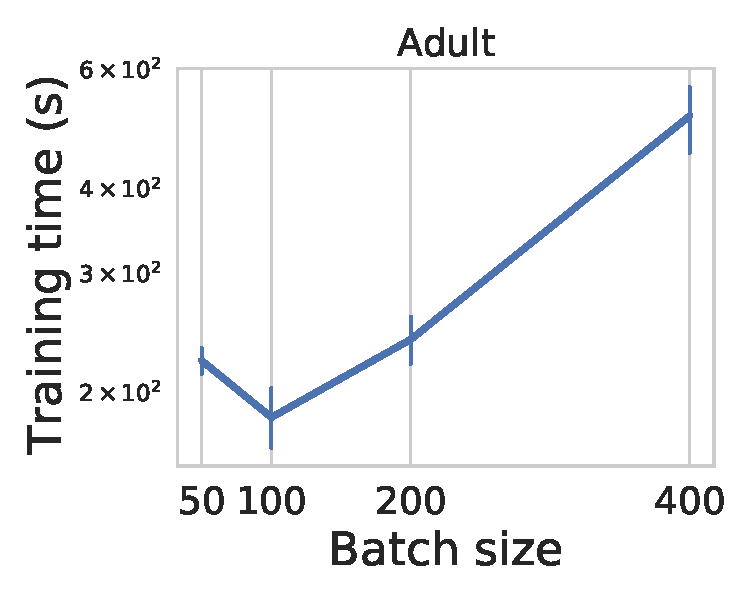
\includegraphics[scale=0.3]{figures/interpretability/imli/batch_size_train_val_fit_time_adult}}
	
	
	
	
	
	\caption[Effect of batch-size in {\imli}]{Effect of bath size on accuracy (test and train), rule-size, and training time. As we consider more samples in a mini-batch, {\imli} generates more accurate and larger size classification rules.}
	\label{interpretability_imli_fig:effect_of_batch_size}
\end{figure}




\begin{comment}


\begin{figure}
	
	
	
	\subfloat{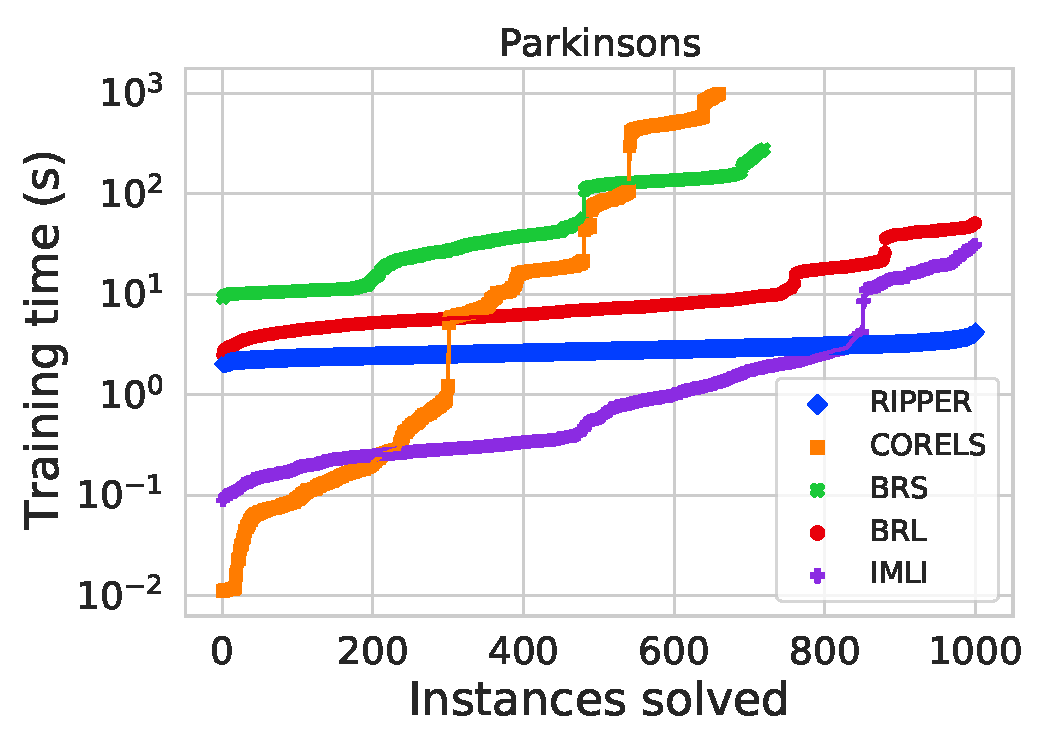
\includegraphics[scale=0.25]{figures/interpretability/imli/dataset_parkinsons_cactus_train_val_fit_time}}
	\subfloat{\includegraphics[scale=0.25]{figures/interpretability/imli/dataset_wdbc_cactus_train_val_fit_time}}
	\subfloat{\includegraphics[scale=0.25]{figures/interpretability/imli/dataset_pima_cactus_train_val_fit_time}}
	
	\subfloat{\includegraphics[scale=0.25]{figures/interpretability/imli/dataset_titanic_cactus_train_val_fit_time}}
	\subfloat{\includegraphics[scale=0.25]{figures/interpretability/imli/dataset_magic_cactus_train_val_fit_time}}
	\subfloat{\includegraphics[scale=0.25]{figures/interpretability/imli/dataset_toms_cactus_train_val_fit_time}}
	
	\subfloat{\includegraphics[scale=0.25]{figures/interpretability/imli/dataset_credit_cactus_train_val_fit_time}}
	\subfloat{\includegraphics[scale=0.25]{figures/interpretability/imli/dataset_adult_cactus_train_val_fit_time}}
	\subfloat{\includegraphics[scale=0.25]{figures/interpretability/imli/dataset_bank_cactus_train_val_fit_time}}
	
	\subfloat{\includegraphics[scale=0.25]{figures/interpretability/imli/dataset_connect_cactus_train_val_fit_time}}
	\subfloat{\includegraphics[scale=0.25]{figures/interpretability/imli/dataset_dota_cactus_train_val_fit_time}}
	\subfloat{\includegraphics[scale=0.25]{figures/interpretability/imli/dataset_weatherAUS_cactus_train_val_fit_time}}
	
	
	\caption{Comparison among interpretable classifiers.}
	\label{interpretability_imli_fig:interpretable_classifiers_all}
\end{figure}


%
%\begin{figure}
%	\subfloat{\includegraphics[scale=0.25]{figures/interpretability/imli/all_datasets_cactus_predicate_count}}
%	\subfloat{\includegraphics[scale=0.25]{figures/interpretability/imli/all_datasets_cactus_test_accuracy}}
%	\subfloat{\includegraphics[scale=0.25]{figures/interpretability/imli/all_datasets_cactus_train_val_fit_time}}
%	\caption{}
%\end{figure}



\end{comment}


%










